\section{Challenge 3: 1 vs 1}

\subsection{Idea of Challenge}
% Patrick
The aim of this challenge is to have some competitive game play given the current situation.   

This challenge focuses on the following aspects:
\begin{itemize}
    \item Remote or autonomous deployment of NAO software and standardised settings for game play in a remote arena on foreign robots
    \item Automatic and semi-automatic calibration of NAO (vision, motion, etc.) 
    \item One versus One NAO competition in a ladder KO competition with all teams without much robot interaction. 
\end{itemize}

Requirements to participate in the scored part of this challenge are being able to
\begin{itemize}
    \item host an arena or have a TODO
    \item deploy your robot's software remotely or fully autonomous setup. 
\end{itemize}

If teams provide an autonomous setup all teams can use this to play against this in their own arena. Also teams who cannot host an arena.

\subsection{Prerequisites}
% Patrick
For this challenge teams need to fulfil multiple requirements, which are listed below in more detail.

First to be able to participate, teams have to be able to deploy their software on the NAO remotely or you can deliver an autonomous setup. There will be several opportunities for the teams to talk, discuss, exchange ideas and code over the next few month until RoboCup. Two options will be properly available: Meetings like RoDEO and an spring RoHOW as well as to discuss on the SPL Discord channel. The second option is a code sharing section as it is available for the V6 support on RC SPL website.  

If teams are not able to participate, they (and the other teams as well) can download and deploy the images for fully autonomous setup, calibration and challenge play in the own lab. These games are not part of the ladder system and are outside of the competition.

\subparagraph*{Basic requirements for teams}

\begin{itemize}
    \item A team must be able deploy their robot software remotely or be able to produce a fully autonomous image for a robot
    \item A team must be able to host an arena. If not they have to find an substitute team, who takes over their hosting arena responsibilities.
    \item A robot should be able to semi- or fully automatic calibrate itself
\end{itemize}

\subparagraph*{Basic requirements for arenas}

The following items have to be fulfilled to be able to host an arena.

\begin{itemize}
    \item A field that is nearly of the size of a approximately 3/4 field or larger.
    \item Field marks as stated in the rules section. 
    \item Two standard goals with nets.
    \item Wifi with standard SPL\textunderscore A session, standard password as communicated during the competition via e-mail and standard IP \texttt{10.0.0.2} address and DHCP turned off.
    \item Remote network access via:
    \begin{itemize}
        \item VPN connection
        \item Mobile connection
        \item TeamViewer or remote desktop connection
    \end{itemize}
    \item Camera, tablet or laptop for on field online calibration with remote team using Discord.
    \item Streaming setup to stream the game on YouTube/Discord/BigBlueButton/Zoom ..., whatever is available (If bandwidth in the lab is limited, an restreaming should be considered on system with better network connection)
    \item Latest Game Controller running. TODO ask BH about 5min and Global Game Stuck button and points 
    \item At least 4 working NAOs V6 per game.
    \item Multiple (>= 4) USB Sticks with 16 GB or more memory for flashing and logging 
    \item At least 4 standard balls.
    \item Assistants for remote setup and autonomous setup
    \item Referees (1 Head, 1 Game Controller Operator, >= 2 Assistants)
\end{itemize}

If you cannot fulfil all requirements but you would like to host an arena, please contact the TC.

\subsection{Arena and organisational setup}
% Patrick
This challenge relies on a standardised arena setup as well as on exchanging all necessary information. This section provides the description for this.

\subsubsection{Data Exchange}
A NextCloud storage is used for data exchange during the days of RoboCup 2021. An access link and password will be sent to the team leaders and have to be used with care. In the NextCloud every team has its own folder (team number) which will be used for sharing the following data:

\begin{itemize}
    \item In folder \textbf{field dimensions} each team has to provide an json file (template will be given) describing the field dimensions according to the rules (TODO: link). The file has to be named \texttt{field\_dimensions.json}. This file has to be uploaded until the 15th of June 2021. The file will be used for autonomous setup and game play. To configure the arena the corresponding field dimensions json will be copied next to the image on the robot as field\_dimensions.json. This allows the usage of the same image at different arenas.
    TODO: Define Json (team name, necessary fields, wifi 5GHz available?)
    \item  In the folder \textbf{field images} each team has a folder where photos from the arena from different angles and at different day \& night times with focus on the lighting conditions get uploaded until the 15th of June 2021.
    \item In \textbf{Robot Setup} the arena teams find an image for a particular game. Each game has an identifier and this identifier should be used as folder name. The image has to be uploaded \textbf{two hours} before the game starts. TODO: Folders
    \item In \textbf{Arena Access} remote teams find an instruction how to access the arena. Each team must provide team specific credentials and share them with the responsible person in each team until the 15th of June. Every teams has to announce a responsible person for credentials and remote setup until the 1st of June. The list of responsible people can be found in the root folder of the NextCloud drive. 
    % TODO: MD File All hosting teams have to sent the TC an email stating that at least 3 other teams were able to setup a robot remotely.
    \item In the root folder you find a \texttt{streaming.md} file where every team should publish a link that can be used by public to watch the game. Will be used on SPL website as well.
    \item Logs and Images will be uploaded from the hosts into the folder \texttt{Logs/Game\_ID}, where \textit{Game\_ID} is replaced by the game identifier, after the game when bandwidth is available. It is assumed that logs and images are stored on the USB drive attached to the NAO in the folder \texttt{logs}. Other files will be ignored. TODO: What is the partition format (NTFS, EXFAT, ...)
\end{itemize}

\subsubsection{Network Setup}
The following section defines network requirements for a venue that hosts remote games. The network infrastructure should be as transparent as possible for remote participants. It should get as close as possible to an on-site experience.

\paragraph{General}

\begin{itemize}
    \item Participants need easy access to their robots for uploading code and debugging. No ports should be blocked. ICMP must not be blocked. TODO: Which ports are necessary?
    \item Robots might accumulate a large amount of log files (including images). These logs will be uploaded after games for analysis. Minimum 100Mbit/s (symmetric) is recommended for a venue, favorable 1Gbit/s. Logs can also be uploaded from another network.
    \item To not overwhelm the network, teams should rate limit their network activity (in particular long log downloads and uncompressed video streams from NAOs during debug sessions)
\end{itemize}

\paragraph{SPL Game specific}

\begin{itemize}
    \item Team Messages (SPLStandardMessages) must be receivable for remote participants
    \item Team Messages must not be forwarded from remote participants to 10.0.0.0/16 (SPL\_A)
    \item GameControllerMessages must be receivable for remote participants
    \item GameControllerMessages must not be forwarded from remote participants to 10.0.0.0/16 to not allow remote participants to control the game (by accident)
\end{itemize}

\paragraph{Example configuration}

\begin{figure}[ht!]
    \centering
    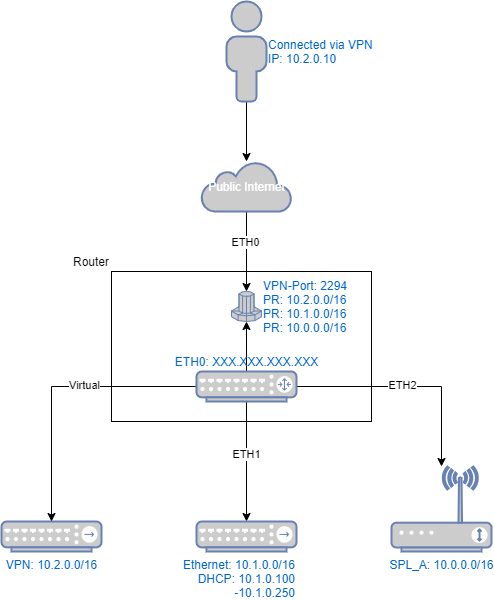
\includegraphics[width=0.5\textwidth]{figs/network.png}
    \caption{Network setup example}
\end{figure}

\begin{itemize}
    \item  The network could be divided for example into three subnets:
    \begin{itemize}
        \item 10.0.0.0/16: The actual SPL\_A wifi network on at least 2.4\,GHz. Each team must use 10.0.TEAM\_NO.2-254 for their robots. GameController will be on 10.0.0.2. DHCP is not active.
        \item 10.1.0.0/16: The ethernet network for robots. Each team must use 10.1.TEAM\_NO.2-254 for their robots. Static addressing is required when robots are assigned to a team. DHCP is active, statically assigning 10.1.0.2-255 to robots that are currently not assigned to any team (pool).
        \item 10.2.0.0/16: The VPN network. Remote participants are assigned to this network and can access the other networks. Team- and GameControllerMessages are forwarded from 10.0.0.0/16 to this subnet. DHCP is active. Broadcasting to other subnets is not possible.
    \end{itemize}
    \item Router (e.g. Edge Router line from Ubiquity)
    \begin{itemize}
        \item serves as router for the whole network.
        \item has a globally routable (and accessible) IPv4 address.
        \item hosts an OpenVPN Layer2 VPN Server
        \item opens a network port to allow incoming OpenVPN connections
        \item Every team gets one certificate to authenticate via OpenVPN (multiple connections allowed).
        \item Has broadcast forwarding rules in place to allow VPN users to receive Team-/GC-Messages.
        \item GameController computer is assigned 10.0.0.2/16
        \item \texttt{ETH0} could be connected to your university network and is preferably accessible from the internet on the specific port (please contact your computer centre how to realise such a connection). If this is not possible, please check if you can make this network accessible from remote using a mobile internet connection. Or you provide a PC connected to an island network of this structure were people can access the PC using Teamviewer, remote desktop software, or something similar. 
    \end{itemize}
\end{itemize}

\subsection{Remote \& Game Setup}
    % - https://writemd.rz.tuhh.de/Tu3JCxovRVunD_yZwBl5Vw#
    % - https://writemd.rz.tuhh.de/rQE55j51QzqO98ifHYF0cQ#
    % - https://writemd.rz.tuhh.de/2YL-Gkz7QX2_zeJyD5Y1jA#

\subsubsection{Start: 2h before match}

    \begin{itemize}
        \item For each team two randomly selected robots are assigned from the pool
        \item Connect robot to LAN and power line
        \item Each robot gets flashed 
        \begin{itemize}
            \item with the standard Softbank image and the LAN IP address is set to 10.1.TEAM\_NO.2 and the replacement robot to 10.1.TEAM\_NO.3, if no individual image is provided by the team.
            \item with the image provided by the teams together with the field\_dimension.json and robot\_id.json indicating if the main robot or the replacement robot gets flashed. (TODO: Create json) TODO: USB Folder
        \end{itemize}
        \item Teams setup robots remotely, if necessary.
    \end{itemize}

\subsubsection{Calibration / Testing: 1 hour before match)}

    \begin{itemize}
        \item 20 min to calibrate the two robots supported by one volunteer from the hosting team. Use for communication the Discord server.
        \item  
    \end{itemize}

    Each team has 1/2 hour on full field for calibration with the help of 1 Volunteer
    Check for wifi
    Check for GC connection

Game setup

    As proposed in special corona rules
    standardized procedure for all teams (Because volunters move robots)
    Referees apply rules to prevent hardware damages (No SBR support probably)
    Longer Pause
    2 preliminary games halves

Game end

    Teams have 10 min to clear robots (may be longer due to limited internet connection)
    Robots are returned to pool
    Next games start



\subsection{Rules}

\subsubsection{Setup of the Environment}
\paragraph{Field Construction}
\label{sec:field_dim}

The soccer field consists of 8mm artificial turf mounted on a flat wooden base with a total area of length \TotalLength and width \TotalWidth.  Care should be taken to ensure the field is as flat and level as possible.  Additionally, the wooden base should be well supported and should not give when humans stand or walk on it.

The dimensions of the soccer field are shown in Figure~\ref{fig:field_dim}.
A more detailed technical drawing is provided in Appendix~\ref{apx:technical-drawing} to this document.

Fields that are at least 3/4 of the original size can also be used for this competition. However, field sizes smaller than the original should be reported by email to the TC by June 1, 2021.
 
Note that the penalty cross is a cross and there is a dash at centre field. White field lines can be made of the same 8mm artificial turf, but in white (\ie, made of white artificial turf), spray painted or taped. Regardless of the solution, the field lines must be durable throughout the competition.

The construction and placement of the goals is depicted in Figure~\ref{fig:goal_dimensions} and Figure~\ref{fig:goal_appearance}. The support structure for the net shall be made with small black, white, or grey bars or cylinders. The support structure shall be constructed exactly as shown in Figure \ref{fig:goal_appearance}.


\begin{figure}[b!]
	\centering
	\centerline{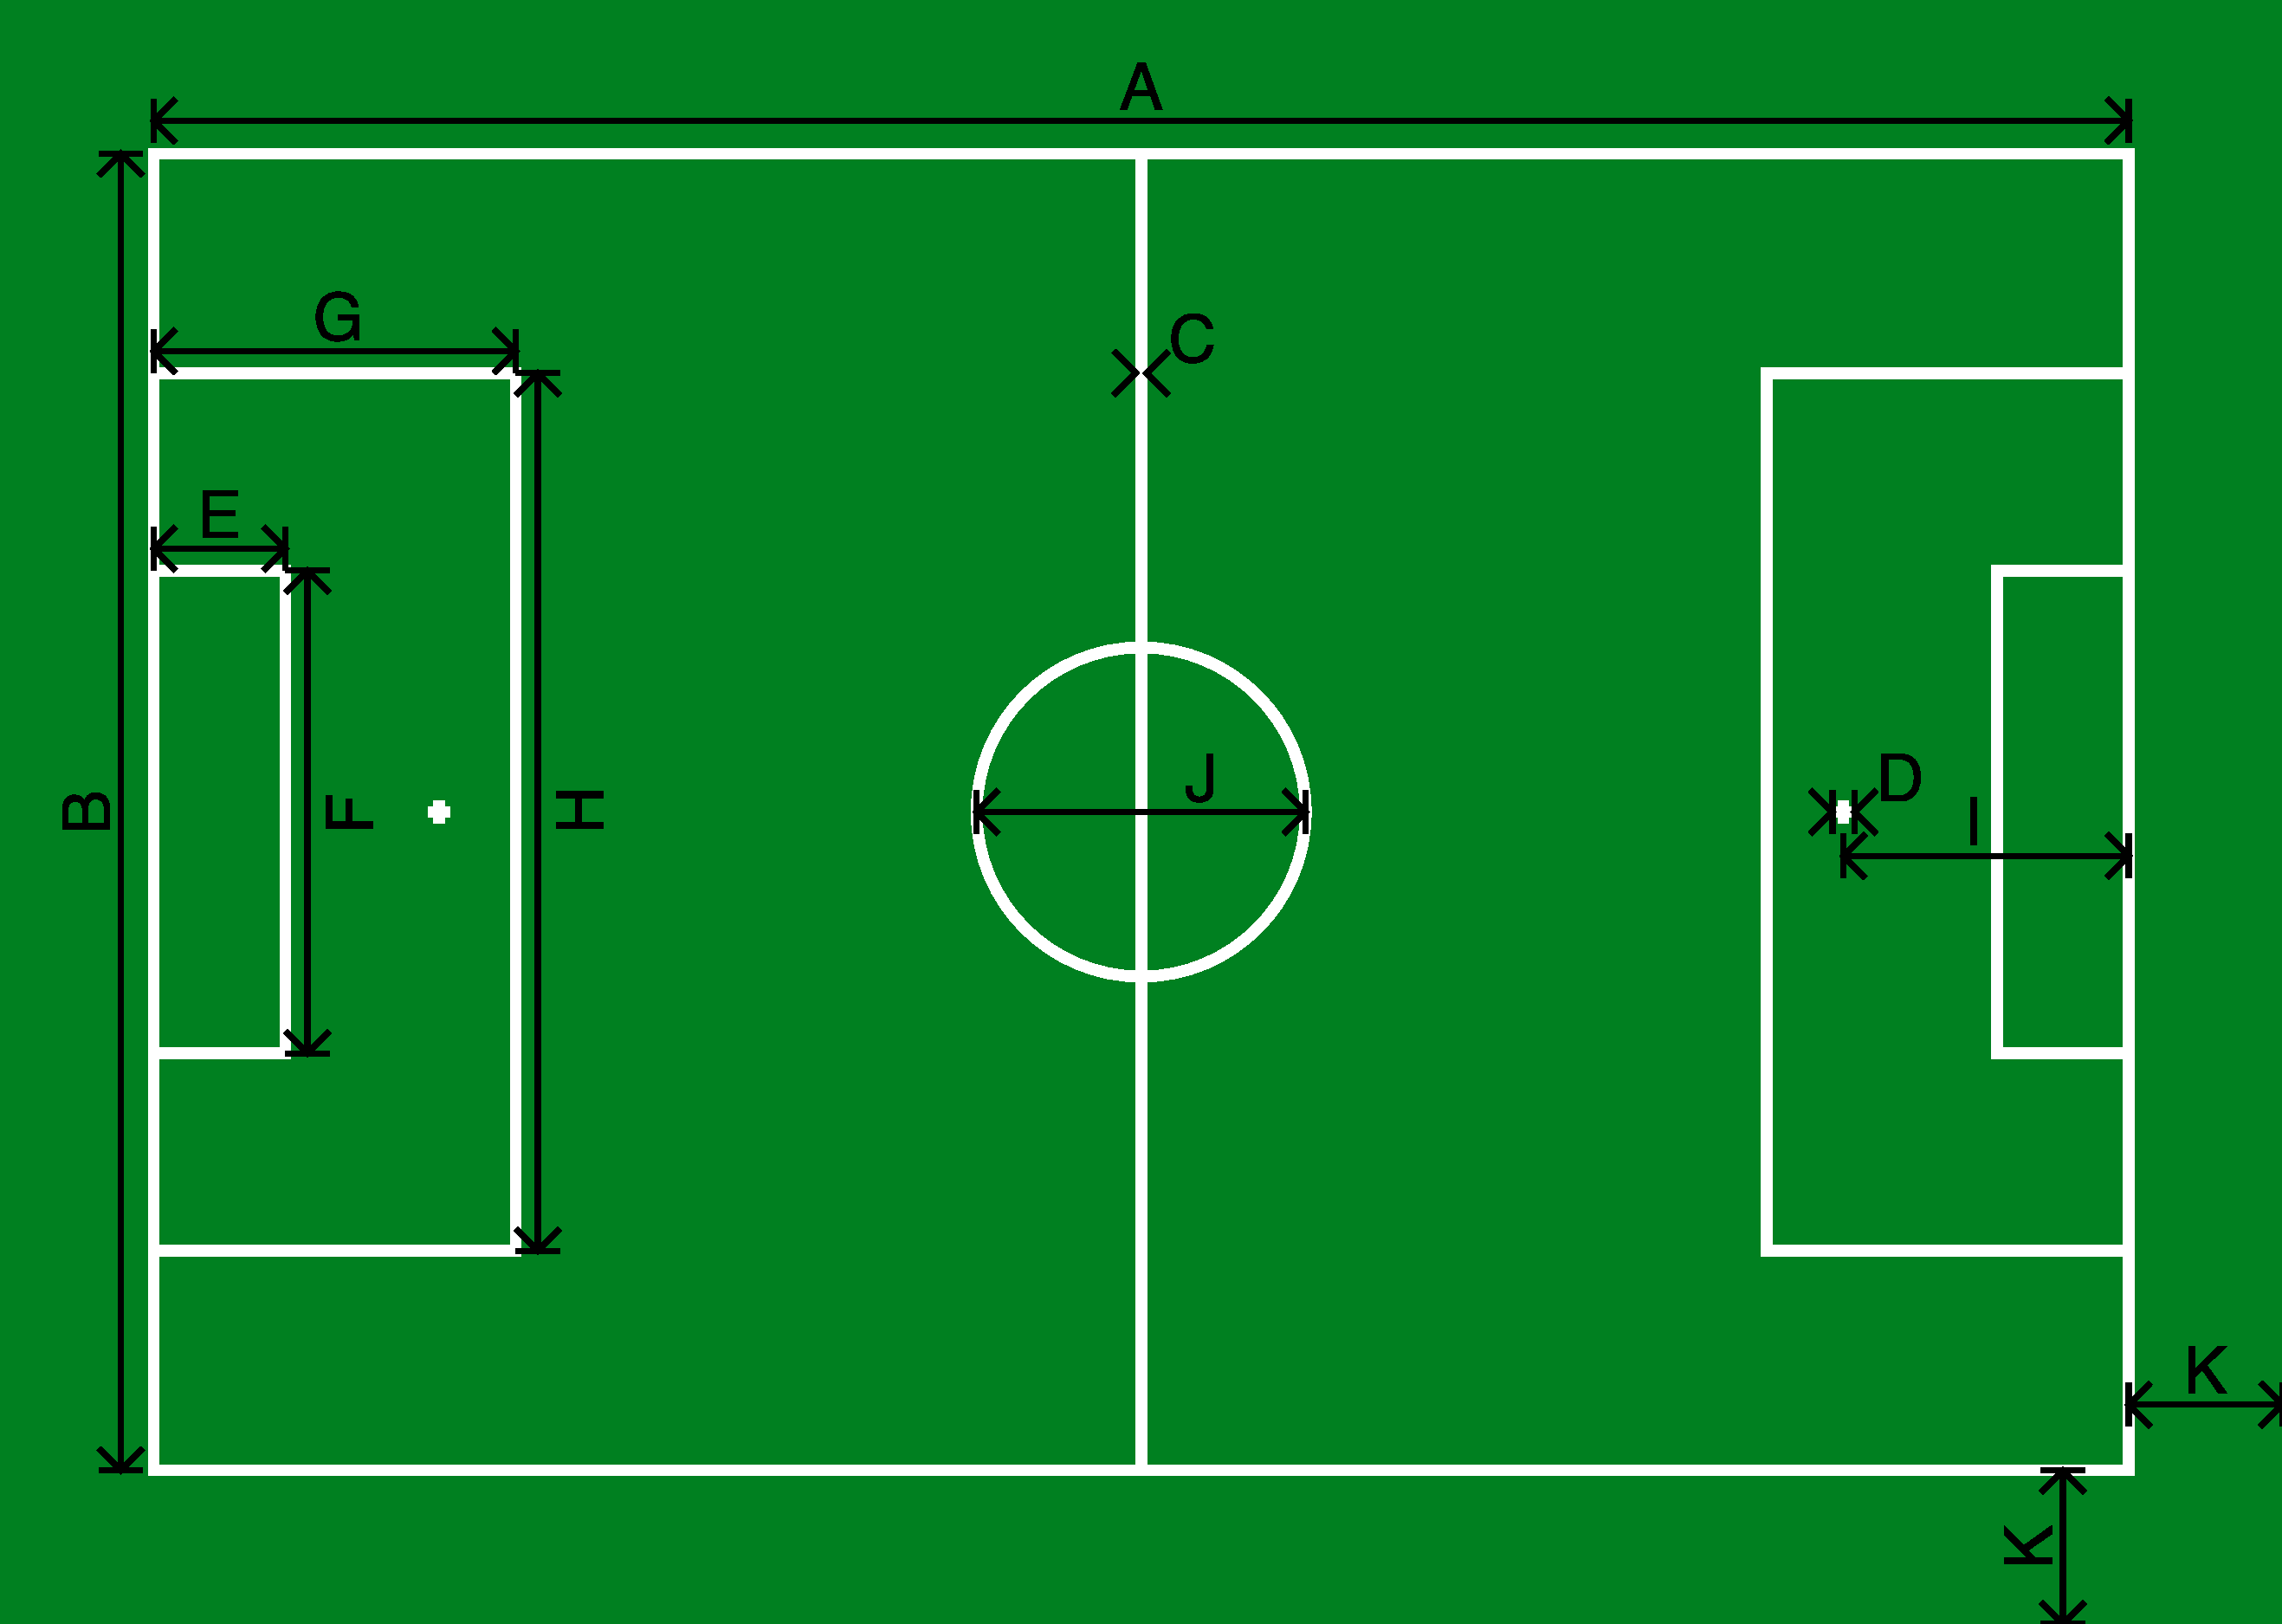
\includegraphics[width=\columnwidth]{figs/fieldDimensions2020.pdf}}
	\vspace{1ex}
	\begin{tabular}{| l | l | l |}
		ID & Description & Length (in mm) \\
		\hline \hline
		A & Field length & 9000 \\
		\hline
		B & Field width & 6000 \\
		\hline
		C & Line width & 50 \\
		\hline
		D & Penalty cross size & 100 \\
		\hline
		E & Goalbox area length & 600 \\
		\hline
		F & Goalbox area width & 2200 \\
	\end{tabular}
	\begin{tabular}{|l|l|l|}
		ID & Description & Length (in mm) \\
		\hline \hline
		G & Penalty area length & 1650* \\
		\hline
		H & Penalty area width & 4000* \\
		\hline
		I & Penalty cross distance & 1300 (1400*) \\
		\hline
		J & Center circle diameter & 1500 \\
		\hline
		K & Border strip width & 700 \\
		\hline
		&  &  \\
	\end{tabular}
	\caption{Schematic diagram of the soccer field (not to scale) and corresponding dimensions in mm. Note that measurements on this diagram are made to the centre of lines. \textcolor{red}{TODO:} Which dimensions are used?
		(*Dimension to be tested and confirmed by May 2020.)} \label{fig:field_dim}
\end{figure}


\begin{figure}[t!]
	\begin{center}
		\leavevmode
		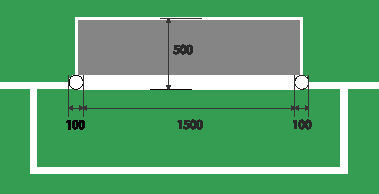
\includegraphics[width=1\columnwidth]{figs/goalDimensions2015.pdf}
		\caption{Dimensions of the goal (in mm), viewed from above, and its placement on the field.}
		\label{fig:goal_dimensions}
	\end{center}
\end{figure}

\begin{figure}[h!]
	\begin{center}
		\leavevmode
		\begin{minipage}[t]{0.49\columnwidth}
			\imagebox{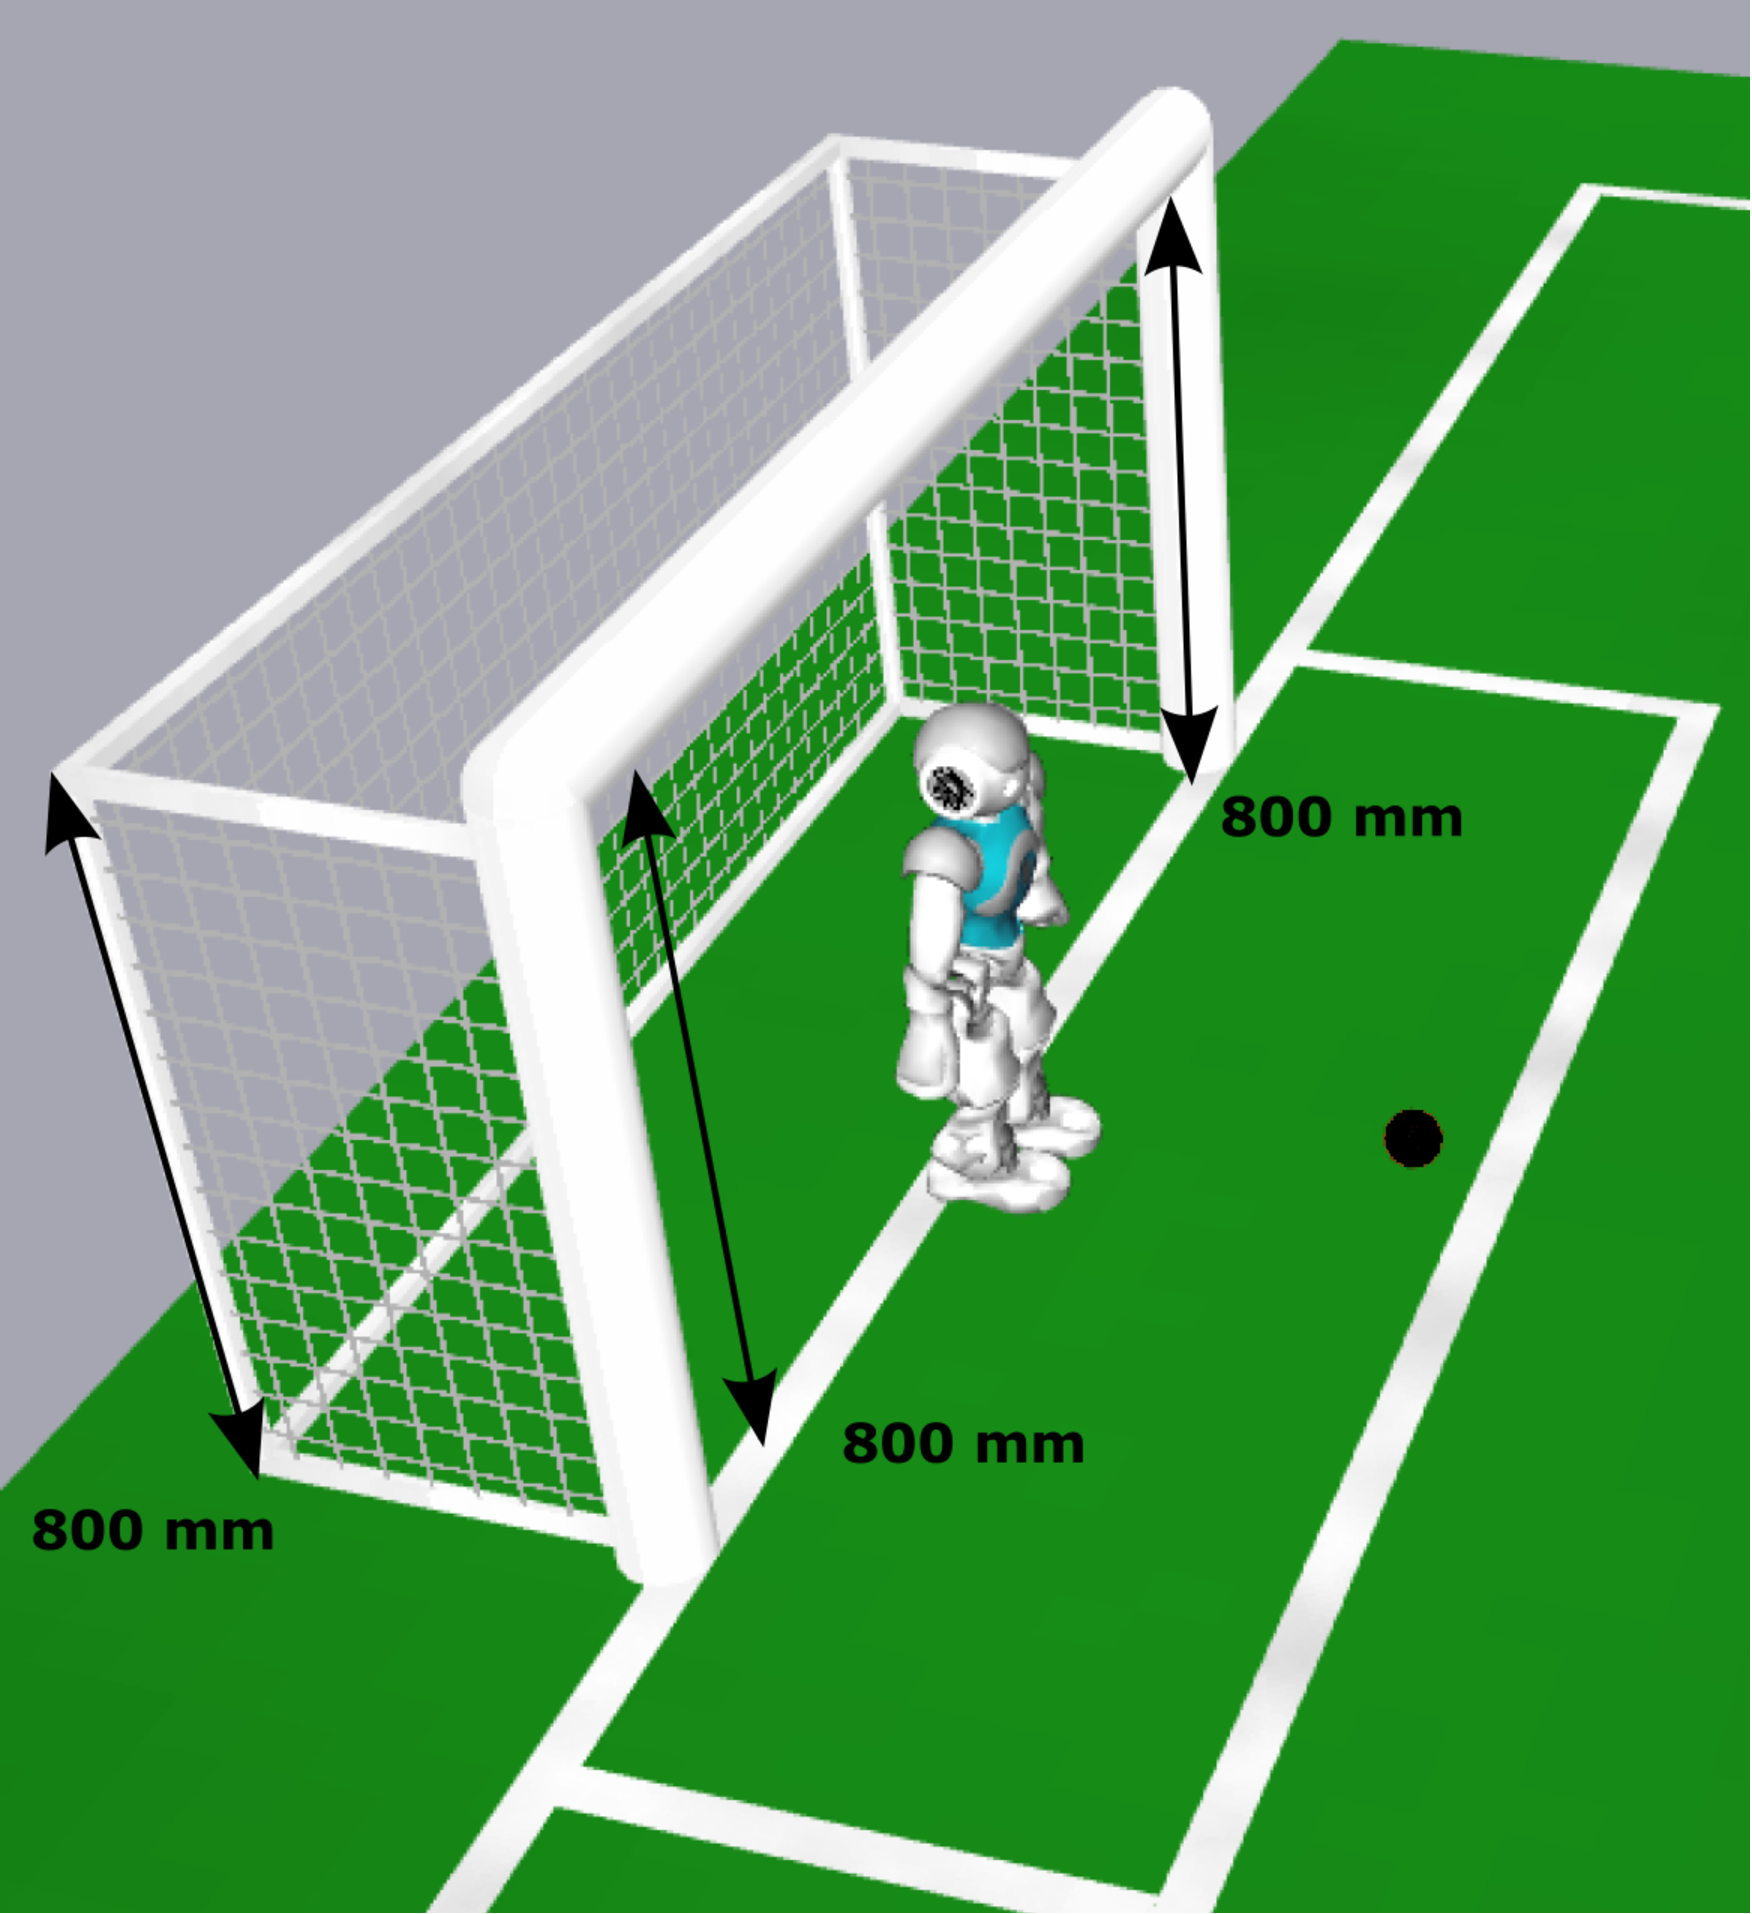
\includegraphics[width=1\columnwidth]{figs/goalDimensions3D.pdf}}%
		\end{minipage}
		\begin{minipage}[t]{0.49\columnwidth}
			The goalposts and crossbar are made from 3 white cylinders with a diameter of 100mm.
			The net:
			\begin{itemize}
				\item has a height of 800mm
				\item is of white, grey or black colour
				\item is tightly supported via the support structure, in a way to minimize interference with the goal keeper
				\item has a weave with holes smaller than the ball diameter.
			\end{itemize}
		\end{minipage}
		\caption{Appearance and dimensions of the goals.}
		\label{fig:goal_appearance}
	\end{center}
\end{figure}

\paragraph{Field Colours}
\label{sec:field_colors}
The colours of the soccer field are as follow:

\begin{itemize}
	\item The field (artificial turf) itself is green (colour is not specified, but it should not be too dark).
	
	\item The lines on the field are white, whether they are taped, spray painted or made from white artificial turf.
	
	\item Goals~(\cf Figure~\ref{fig:goal_appearance}). The posts and top cross bar of both goals are white. The net and the support structure for the net are white, grey, or black.
\end{itemize}

\paragraph{Lighting Conditions}
\label{sec:lightConditions}
The lighting conditions depend on the actual competition site. As the league moves towards natural lighting conditions, SPL fields should be placed near or under windows where possible. Whether or not window lighting is used, ceiling lights should be provided as necessary to ensure that most of the field is never darker than 300 Lux (400 Lux preferred).

Lighting is not required to be even and hotspots may occur on the field. The lighting design (comprising both natural and artificial light sources) shall aim to limit the ratio between the brightest and darkest patches on the field to less than 10:1. In general, lighting irregularities, including changes that occur during the competition, are acceptable and will not be cause for delay. Such irregularities may include sun streaming through windows, light bulbs turning off, light bulbs being replaced, etc.

\paragraph{Ball}
\label{sec:ball}

The official ball is a soft foam ball with a black and white soccer ball print (see Figure~\ref{fig:ball}). They are 100mm in diameter and weigh 44 grams. These balls are available by writing to \url{info@sportpaint.de} (in German or English) and asking to order the "pu schaumstoffball 10cm 100ss".  Each ball costs EUR 2.50 plus shipping, where shipping cost depends on the destination.

\begin{figure}[t]
	\centerline{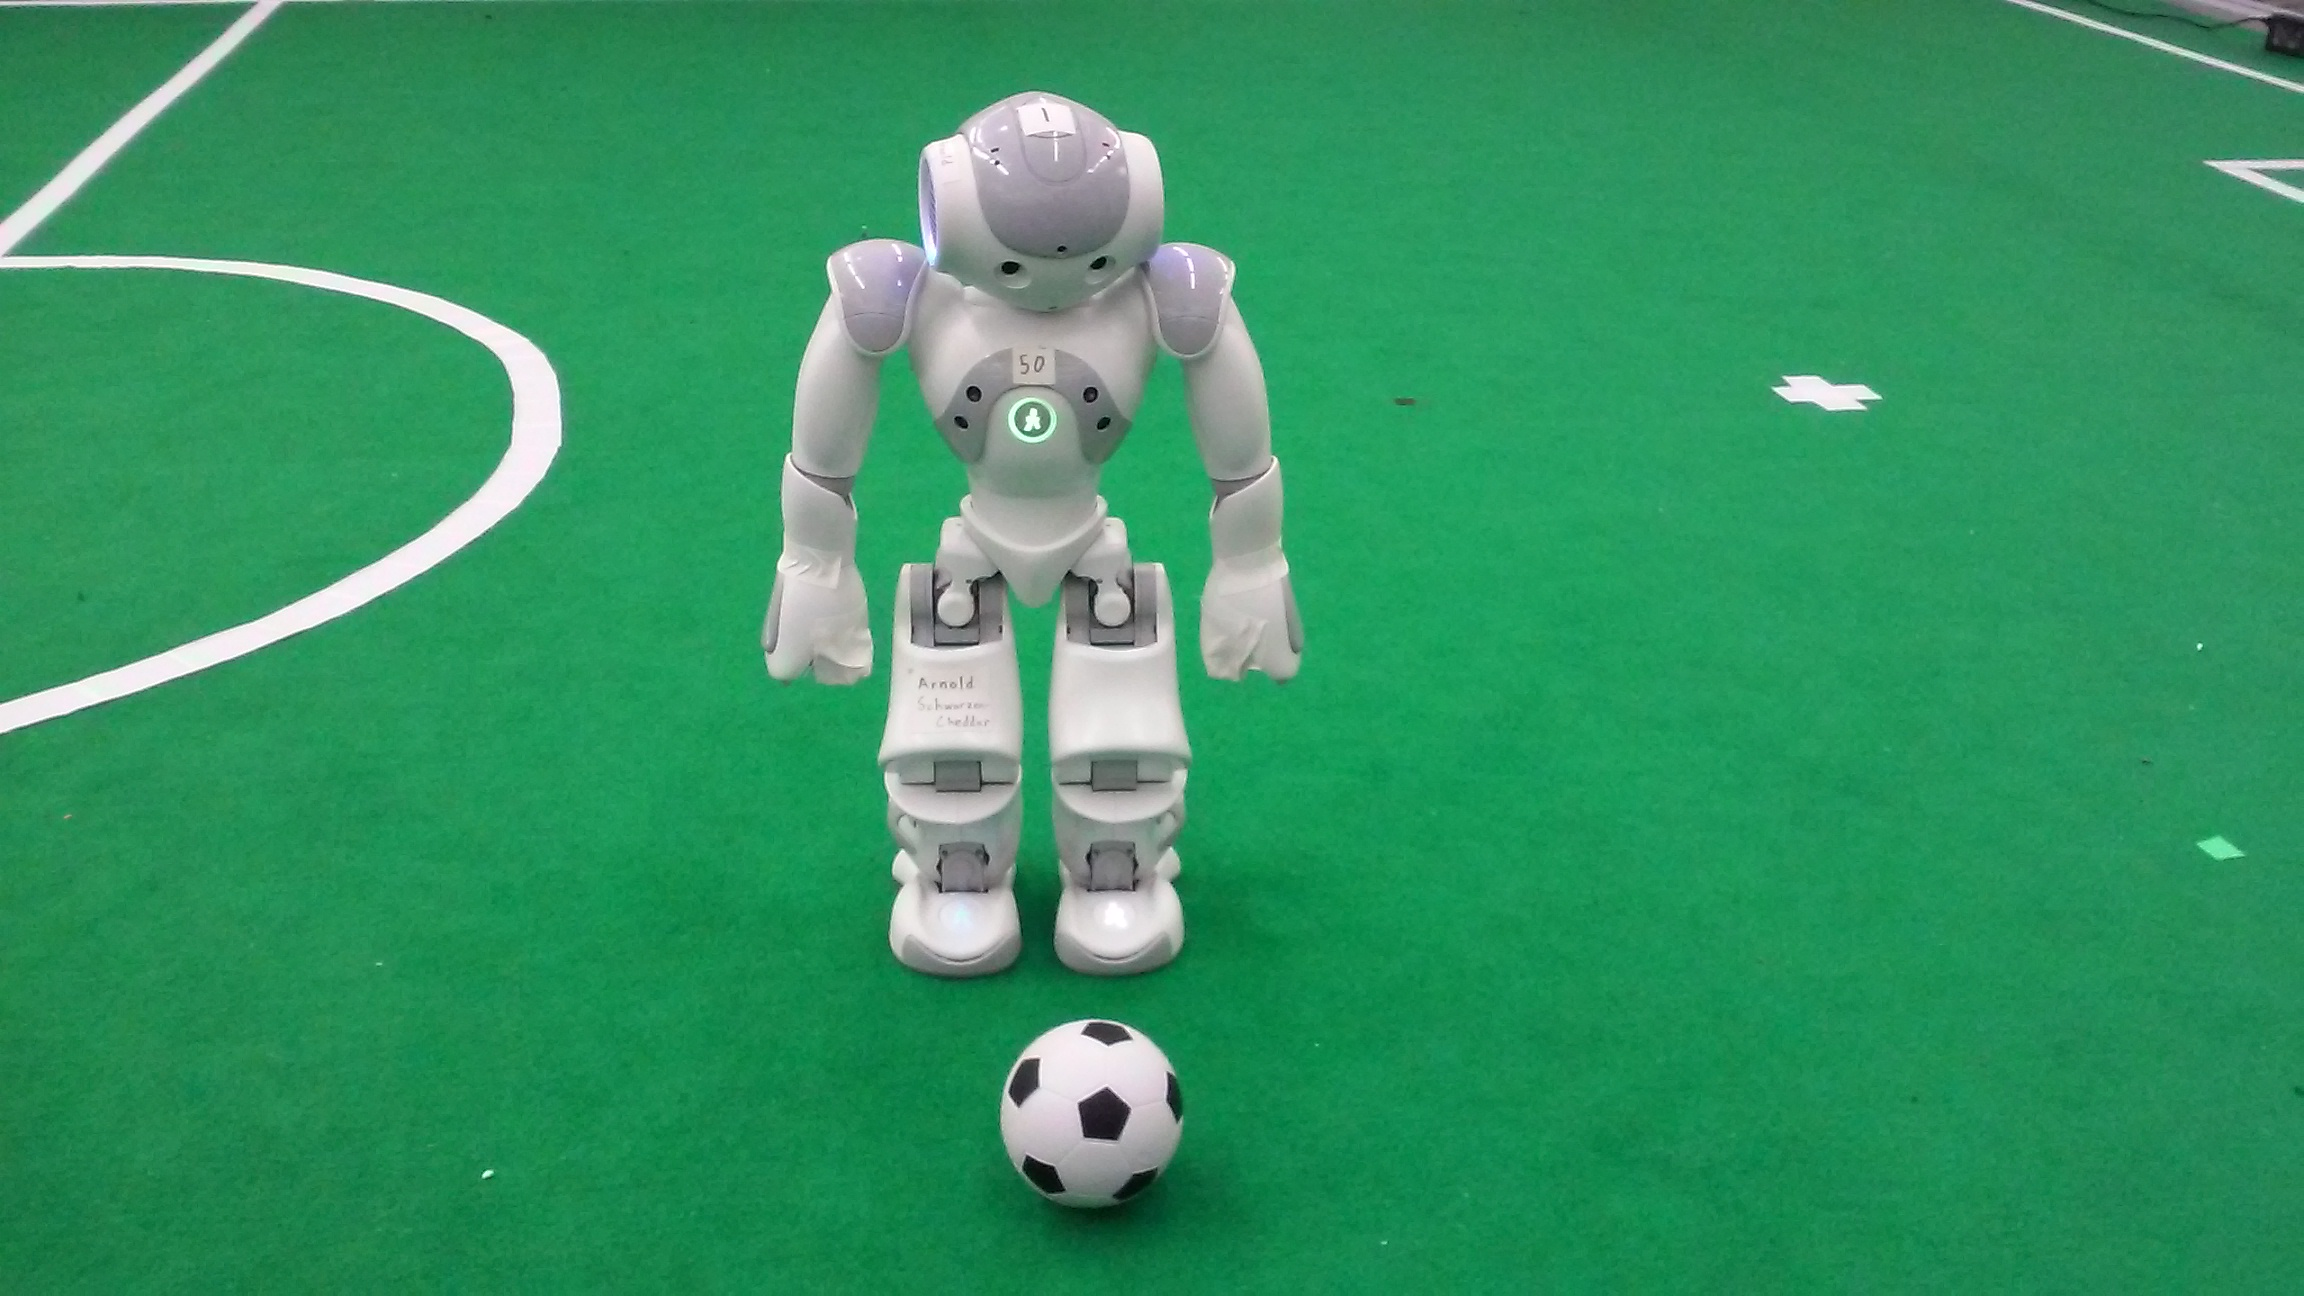
\includegraphics[height=0.28\columnwidth]{figs/robotWithBall2016.jpg}}
	\caption{A NAO and the official ball.}
	\label{fig:ball}
\end{figure}


\paragraph{Definition of Inside and Outside}
\label{sec:inside_outside}

A line is always part of a region of the field.
This means, that \emph{inside/outside \textless region\textgreater} refers to the green area as well as the surrounding line.
Specifically:
\begin{itemize}
	\item The field boundary lines are part of the field
	\item The penalty box lines (and the end field line inside of the goal) part of the penalty box
	\item The centre circle lines are part of the centre circle
\end{itemize}

The only \textit{exception} to this rule is the centre field line, which does not form part of any half.
That is, a robot is \textit{outside} of a half of the field if it is touching the centre line.

\newpage


\subsubsection{Robot Players}
\label{sec:robot_players}
A match is played by two teams, each consisting of \emph{one player} and \emph{one substitute player}. All robots are \emph{field players} and no robot is designated as \emph{goalkeeper}.

\paragraph{Hardware}
\label{sec:hardware}
All teams must use a NAO humanoid robots in version 6 manufactured by SoftBank Robotics.

Absolutely no modifications or additions to the robot hardware are allowed. No additional hardware is permitted including off-board sensing or processing systems. Additional sensors besides those originally installed on the robots are likewise not allowed. The only exceptions are:
\begin{itemize}
	\item Setting the passive wrist joints to a fixed position either with glue or a transparent or white duct tape.
	\item Protecting the fingers with white finger protectors provided by the manufacturer or with transparent or white duct tape.
	\item Placing white duct tape over the battery case and screw (under the robot jersey) to keep the battery case in place and prevent the battery becoming disconnected.
	\item A memory stick may remain in the head during operation.  Only ordinary USB flash memory keys that sit flush or recessed to the head casing may be utilized. Other USB dongles or devices, as well as memory sticks that are not flush or recessed, are not permitted.
\end{itemize}

\paragraph{Field Players}
\label{sec:field_players}
Each field player has a jersey number from the set $\{1, 2, 3, 4, 5, 6\}$. However, by default, the number ``2'' is used for the first field player and the number ``3'' should be used for a substitute that enters the game later. This assignment can be changed due to availability of jerseys.

\paragraph{Team Markers}
\label{sec:team_markers}
Robots use coloured jersey shirts as team markers in the ``home'' and ``away'' colours of the hosting arena team. Each jersey shirt has a player number (1-6) printed on it. The team markers are worn as shown in Figure~\ref{fig:nao_markers}.

\begin{figure}
	\centerline{\begin{tabular}{lll}
			a) & b) & c) \\
			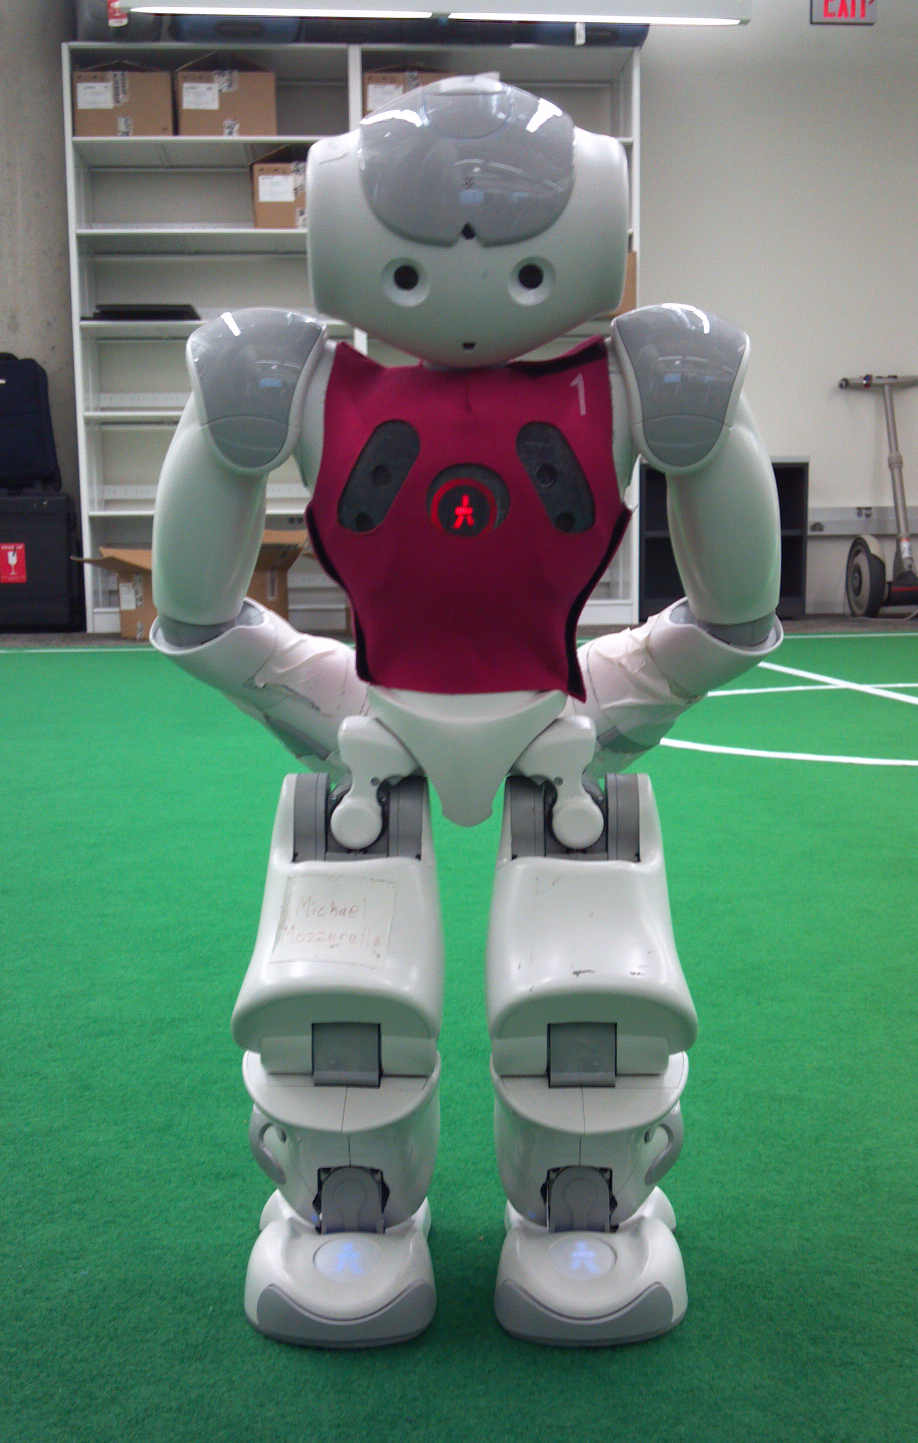
\includegraphics[height=0.28\columnwidth]{figs/front.jpg}&
			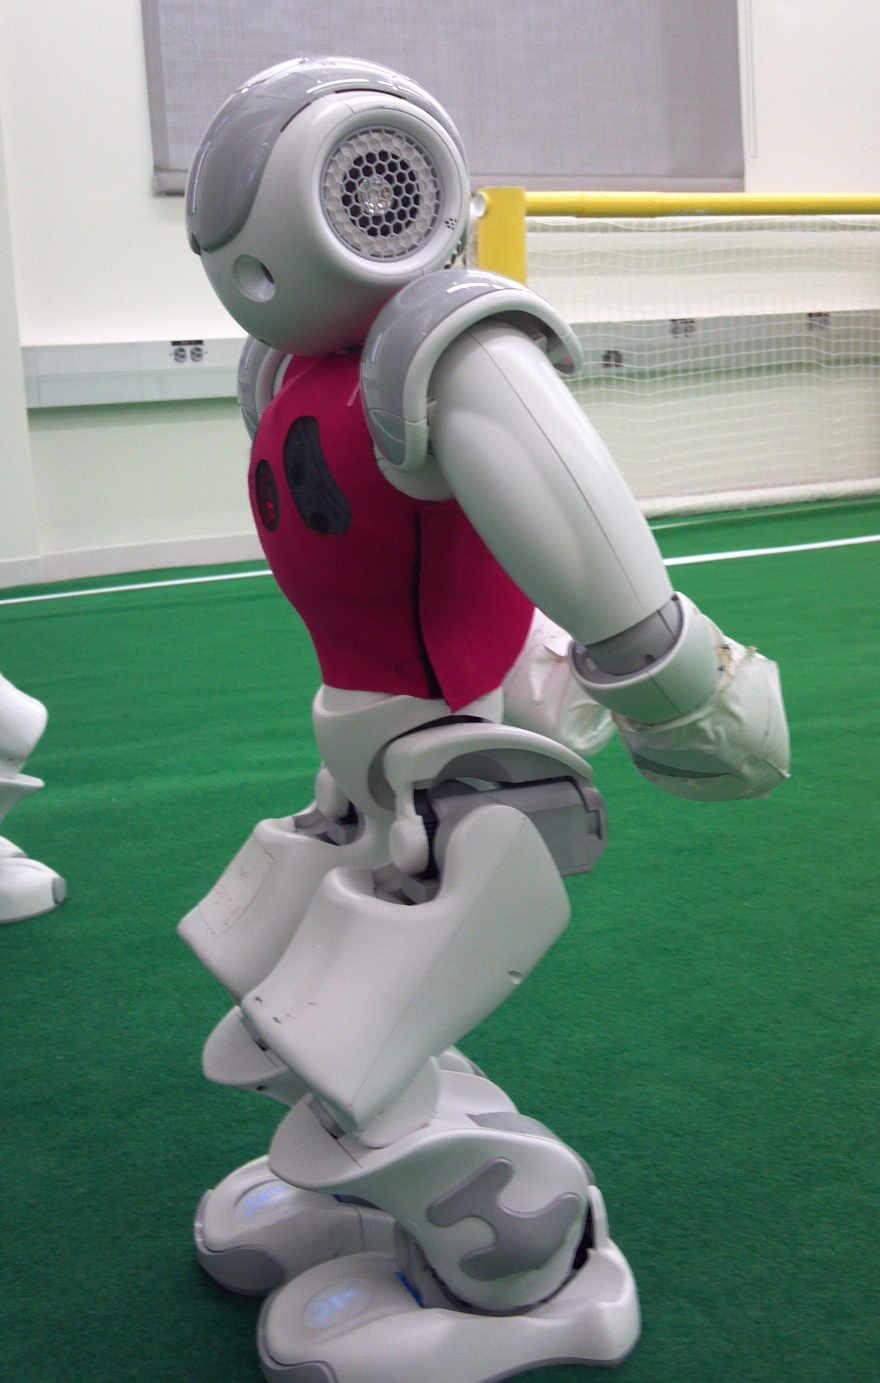
\includegraphics[height=0.28\columnwidth]{figs/side.jpg} &
			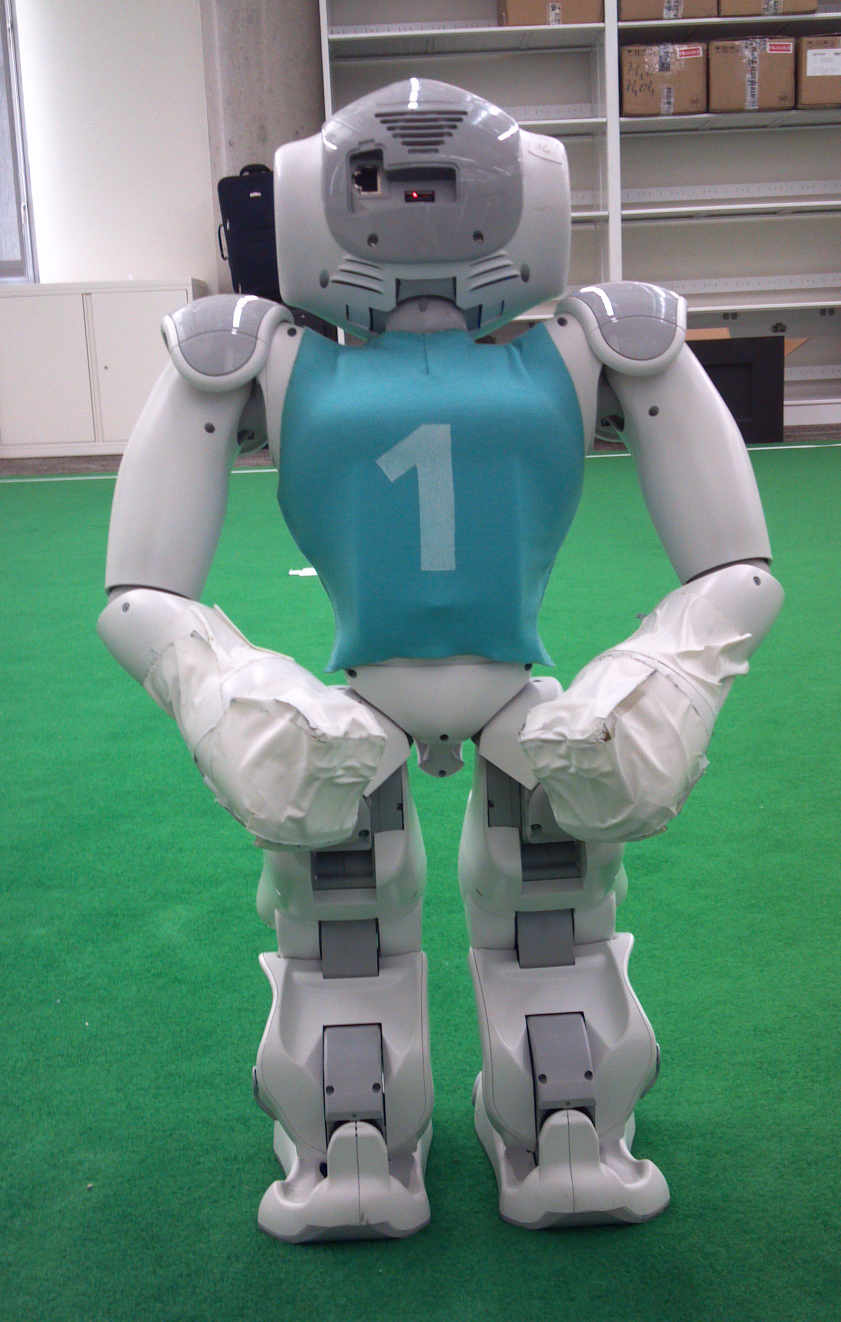
\includegraphics[height=0.28\columnwidth]{figs/back.jpg}
	\end{tabular} }
	\caption{Team markers. a) Front view. b) Side view. c) Back view.}
	\label{fig:nao_markers}
\end{figure}


Teams may design and manufacture their own jerseys in any colour (multi and many colour jerseys are acceptable), but must follow these guidelines:
\begin{itemize}
	\item Jerseys should be the tank top style used at RoboCup 2013/2014 and should cover approximately the same areas of the robot as shown in Figure~\ref{fig:nao_markers}.  The torso LED must be clearly visible.  Jerseys may include the sonar panel used in the 2013/2014 jerseys, although this is not required.
	\item Jerseys must have a primary colour that comprises at least 70\% of the jersey.
	\item Jerseys should not contain distractors, such as large pictures of SPL balls or white stripes on green jerseys.
	\item All players on a team must wear identical jerseys.
	\item A team must wear the jerseys that it starts a game in for the entire game.
	\item Jersey material must be non-reflecting, non-shiny, and non-textured.  Material that is glittery is also not appropriate.
	\item Jerseys should be numbered 1-6 on both sides.  The numbers must be large and {\bf easily} recognized by humans.
	\item Teams must have two sets of jerseys that are significantly different in terms of their primary colour.
	\item Designs must be submitted to \url{rc-spl-tc@lists.robocup.org} for approval by May 1st, 2021. If the team has jersey prototypes, they should submit close-up images of a robot wearing the jersey - these images should be taken from front, back, and side angles.  If the team has no prototypes, then designs depicting the expected jersey should be submitted.  If submissions show separated front and back halves of jerseys then the team must specify which halves are matched to form home and away jerseys.  All images and designs should be submitted in pdf or jpg format.
\end{itemize}

Each team/arena must designate a ``home'' colour and an ``away'' colour when asked about one month before RoboCup. Robots must wear the `home' jerseys when they are ``home'' (the first team listed on the schedule). The ``away'' team (the second team listed on the schedule) will wear the ``away'' jerseys.

Some teams wish to include additional information or logos on their robots.  The following are allowable:
\begin{itemize}
	\item Attaching player numbers to the heads and/or legs of the robots.  These numbers should be black with a white background, and should correspond to the number on the robot's jersey.
	
	\item Adding sponsor or team logos to the upper legs of the robots (\cf Figure~\ref{fig:sponsor}). A box drawn around the non-white area of these logos must not cover more than a 25 $\text{cm}^2$ area. At most one logo may be attached per leg --- if you wish to attach more than one logo per leg, email the Technical Committee at least two weeks before the competition.  Depending on the size and design of the logos, this may be allowable.
	
	\item Adding small black and white stickers to the torso of the robots stating the name of the robot, the name of the team, or similar information. These stickers must be small and mostly white.
\end{itemize}

\begin{figure}[b]
	\centerline{\begin{tabular}{ll}
			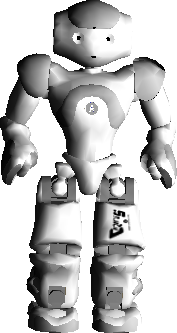
\includegraphics[height=0.35\columnwidth]{figs/naosim_with_logo.png}&
			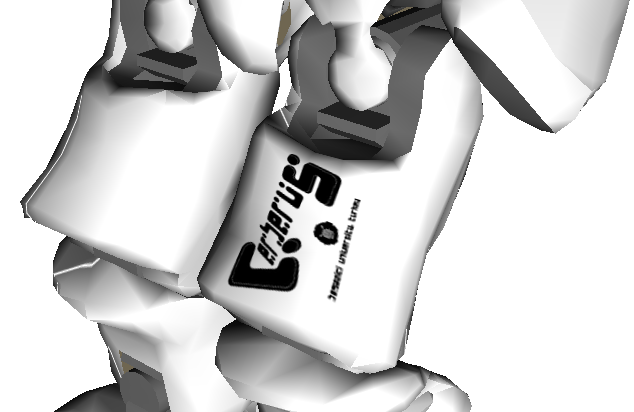
\includegraphics[height=0.35\columnwidth]{figs/naosim_legs_with_logo_closeup.png}
	\end{tabular}}
	\caption{Example Sponsor/Team Logo placement on legs.}
	\label{fig:sponsor}
\end{figure}

\paragraph{Wireless Communications}
\label{sec:wireless}
The robots must play without human control. Communication is only allowed between a robot and the GameController.

The only wireless hardware allowed to be used by the teams/arenas are the wireless network cards built into the NAOs, and the access points provided by the arena. All other wireless hardware must be deactivated. A team/arena may be disqualified if one of the team members violates this rule.

Each team will get a range of IP addresses that can be used both for their robots and their computers/remote connections. The network configuration (\eg IP addresses, channels, SSIDs, and required encryption) of the fields will be announced by the arena. 

%TODO: reference default configuration

Teams and their robots must not listen into another team's communication.

The GameController will use UDP to connect to the robots. The source distribution of the GameController provides the header file \emph{RoboCupGameControlData.h} that defines all messages sent by the GameController to the robots. They correspond to the \emph{robot states} described in Section~\ref{sec:robot_states}.

Robots send status updates (defined in \emph{RoboCupGameControlData.h}) to the GameController. These return packets must be addressed directly to the GameController PC (\ie not broadcast) and sent on the GameController return UDP port specified by the symbol \verb!GAMECONTROLLER_RETURN_PORT! in \emph{RoboCupGameControlData.h}.

The use of remote processing/sensing is prohibited.

\newpage

\subsubsection{Game Process}
\label{sec:game_process}

\paragraph{Structure of the Competition}
\label{sec:game_struct}

A 1vs1 competition consists of three parts, the first half, a half-time break, and the second half. Each half is 5 minutes counted from the initial kick-off.
The half-time break is five minutes and during this time both teams may change their robot to the substitute player, but code changes are prohibited in the half-time. It is mainly used to cool down the robots and to charge them. 

The head referee signals the commencement of each half with a single whistle blow (that is, the Initial kick-off, \cf Section~\ref{sec:initial-kick-off}).
The head referee signals the end of the first half with two short whistle blows, and the end of the second half with two short plus one long whistle blow.
The head referee should make \textit{all} of these whistle sounds from the T-junction of the half-way line.

The teams/robots will change the goal defended during the half-time break.

\paragraph{Robot States}
\label{sec:robot_states}

Robots can be in six different \emph{primary} states (\cf Figure~\ref{fig:robot_states}). If the wireless is available, these states will be set by the GameController. Teams must implement code to receive and correctly respond to wireless GameController packets, and also give a visual indication of the game state.

\textbf{The use of the button interface is not allowed in this competition!} 

Should both robots have problems with the Wifi/GameController connection the head referee should issue a referee timeout (\cf Section~\ref{sec:referee_timeout}).
If only one robot does not respond to the GameController then it is not included in the game (via a `Request for Pick-up'), and the game starts without the offending robot.
%TODO: RFP reference

\begin{description}
	\item[Initial.] After booting, the robots are in their \emph{initial} state. The robots are not allowed to be moving in any fashion besides initially standing up. Shortly pressing the chest button will switch the robot to the \emph{penalized} state.
	
	\item[Ready.] In this state, the robots walk to a legal position on their half. They remain in this state, until the head referee decides that there is no significant progress, up to a maximum of \KickOffAutoTime.
	
	\item[Set.] In this state, the robots stop and wait for Kick-Off  (\cf Section~\ref{sec:kick-off}).
	Illegally positioned robots are penalized.
	Robots are allowed to move their heads or get up if fallen before the game (re)starts but they are not otherwise allowed to move their legs or locomote in any fashion.
	If a robot cannot get up, fallen robot is called~(\cf Section~\ref{sec:fallenrobots}).
	The penalty time counter is frozen during this state.
	Note that all penalized robots are left in place (on the side of the field, or in-place for motion in set) and must wait to get unpenalized.
	
	\item[Playing.] In the \emph{playing} state, the robots are playing the 1vs1 competition.
	
	\item[Penalized.] A robot is in this state when it has been penalized. It is not allowed to move in any fashion,  this includes stopping the head turning.
	
	\item[Finished.] This state is reached when a half is finished.
\end{description}

\begin{figure}[t]
	\centerline{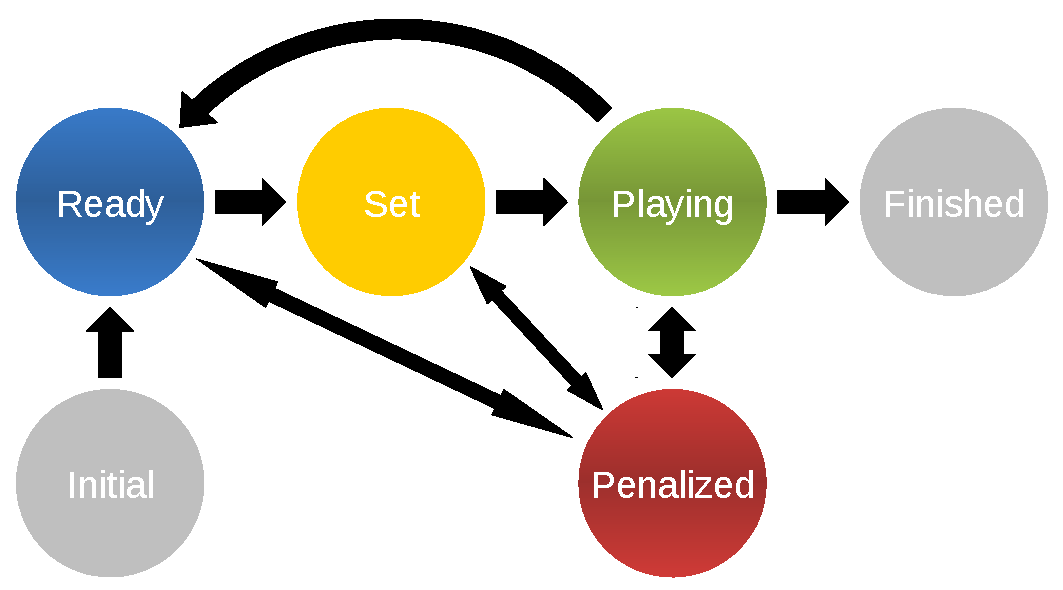
\includegraphics[width=0.9\columnwidth]{figs/states.pdf}}
	\caption{Robot states. GameController transitions are shown in black. However, any transition possible for this competition is only sent by the GameController.}
	\label{fig:robot_states}
\end{figure}

The referee will announce the start of the Playing state with a single whistle blow.
The GameController Playing signal will be delayed by \PlayingDelayTime.
Robots that begin moving their legs or locomoting in any fashion during \emph{set} (\ie before the referee blows the whistle) will be penalized \textit{in place} on the field via the ``Motion in Set'' (\cf Section~\ref{sec:motion_in_set}) GameController signal (and moved back to their original position if they have moved significantly before becoming penalized) until the GameController transmits the \emph{Playing signal}.

The current game state should be displayed on the LED in the torso. The colours corresponding to the game states are:

\begin{itemize}
	
	\item Initial: Off
	
	\item Ready: Blue
	
	\item Set: Yellow
	
	\item Playing: Green
	
	\item Penalized: Red
	
	\item Finished: Off
	
\end{itemize}

The current GameController requires robots to know both their team number and their robot number within the team. It is each team's responsibility to make sure this is correctly configured. It is recommended that the robot indicates its number within the team on bootup so that this can be easily checked at the start of the game.

\paragraph{Goal}
\label{sec:goal}
A goal (including own goal) is achieved when the entire ball (not only the centre of the ball) goes over the goal-side edge of the goal line, \ie the ball is completely inside the goal area\footnote{The goal line is part of the field.}. \\
If a player (from both sides) scores a valid goal the ball gets replaced by the referees to one of the starting points, on the other half, that is farthest away from the player in this half. The ball can then directly be played again. 
%TODO: Reference -> points.

The head referee signals a goal by a single whistle blow, followed by the call ``Goal \textless colour\textgreater''. However no GameController action shall be performed. \textcolor{red}{TODO}: Maybe we an change the logic of the GameController to allow for counting goals without ready and set phase. \\
After the game is in the state playing, the game state remains in it regardless of shot goals!


\paragraph{Initial Kick-off}
\label{sec:initial-kick-off}

The first kick-off at the start of each half is the initial kick-off.
Before the initial kick-off, \ie before the start of each half, both robots must be in the initial state and must be placed on the sidelines, closest to the GameController, in their own half of the field at the height of the penalty spot. 
Once the robots receive the \emph{ready} signal from the GameController, they are to proceed as described in Section~\ref{sec:kick-off}.

\paragraph{Kick-off}
\label{sec:kick-off}
For kick-off, the robots listening to the wireless GameController run through three states: \emph{ready}, \emph{set}, and \emph{playing}. It is to a team's responsibility to have their robots listen to the GameController!

In the ready state, the robots should walk to their legal kick-off positions.
The players can be positioned anywhere within their own half, but no player is allowed to touch the centre/halfway line. All robots that do not reach legal positions will be penalized with the ``Illegal Position'' penalty~(\cf Section~\ref{sec:illegal_positioning}).

In the \emph{set} state, the robots must not locomote~(\cf Section~\ref{sec:robot_states}). A referee places the two balls for each side on the goal free kick positions.%TODO:Reference
If the ball is moved by one of the robots during \emph{set} it is replaced by one of the referees.

\textcolor{red}{TODO}:Allow manual placement or simplify the rules without it?
%During the \textit{set} state, the team leader may request manual placement for all robots on that team --- including those penalized in place for ``Motion in Set'' but not those with other penalties. Note that the, ``Motion in Set'' penalty persists for those players after manual placement.

%\begin{figure}[t]
%	\centerline{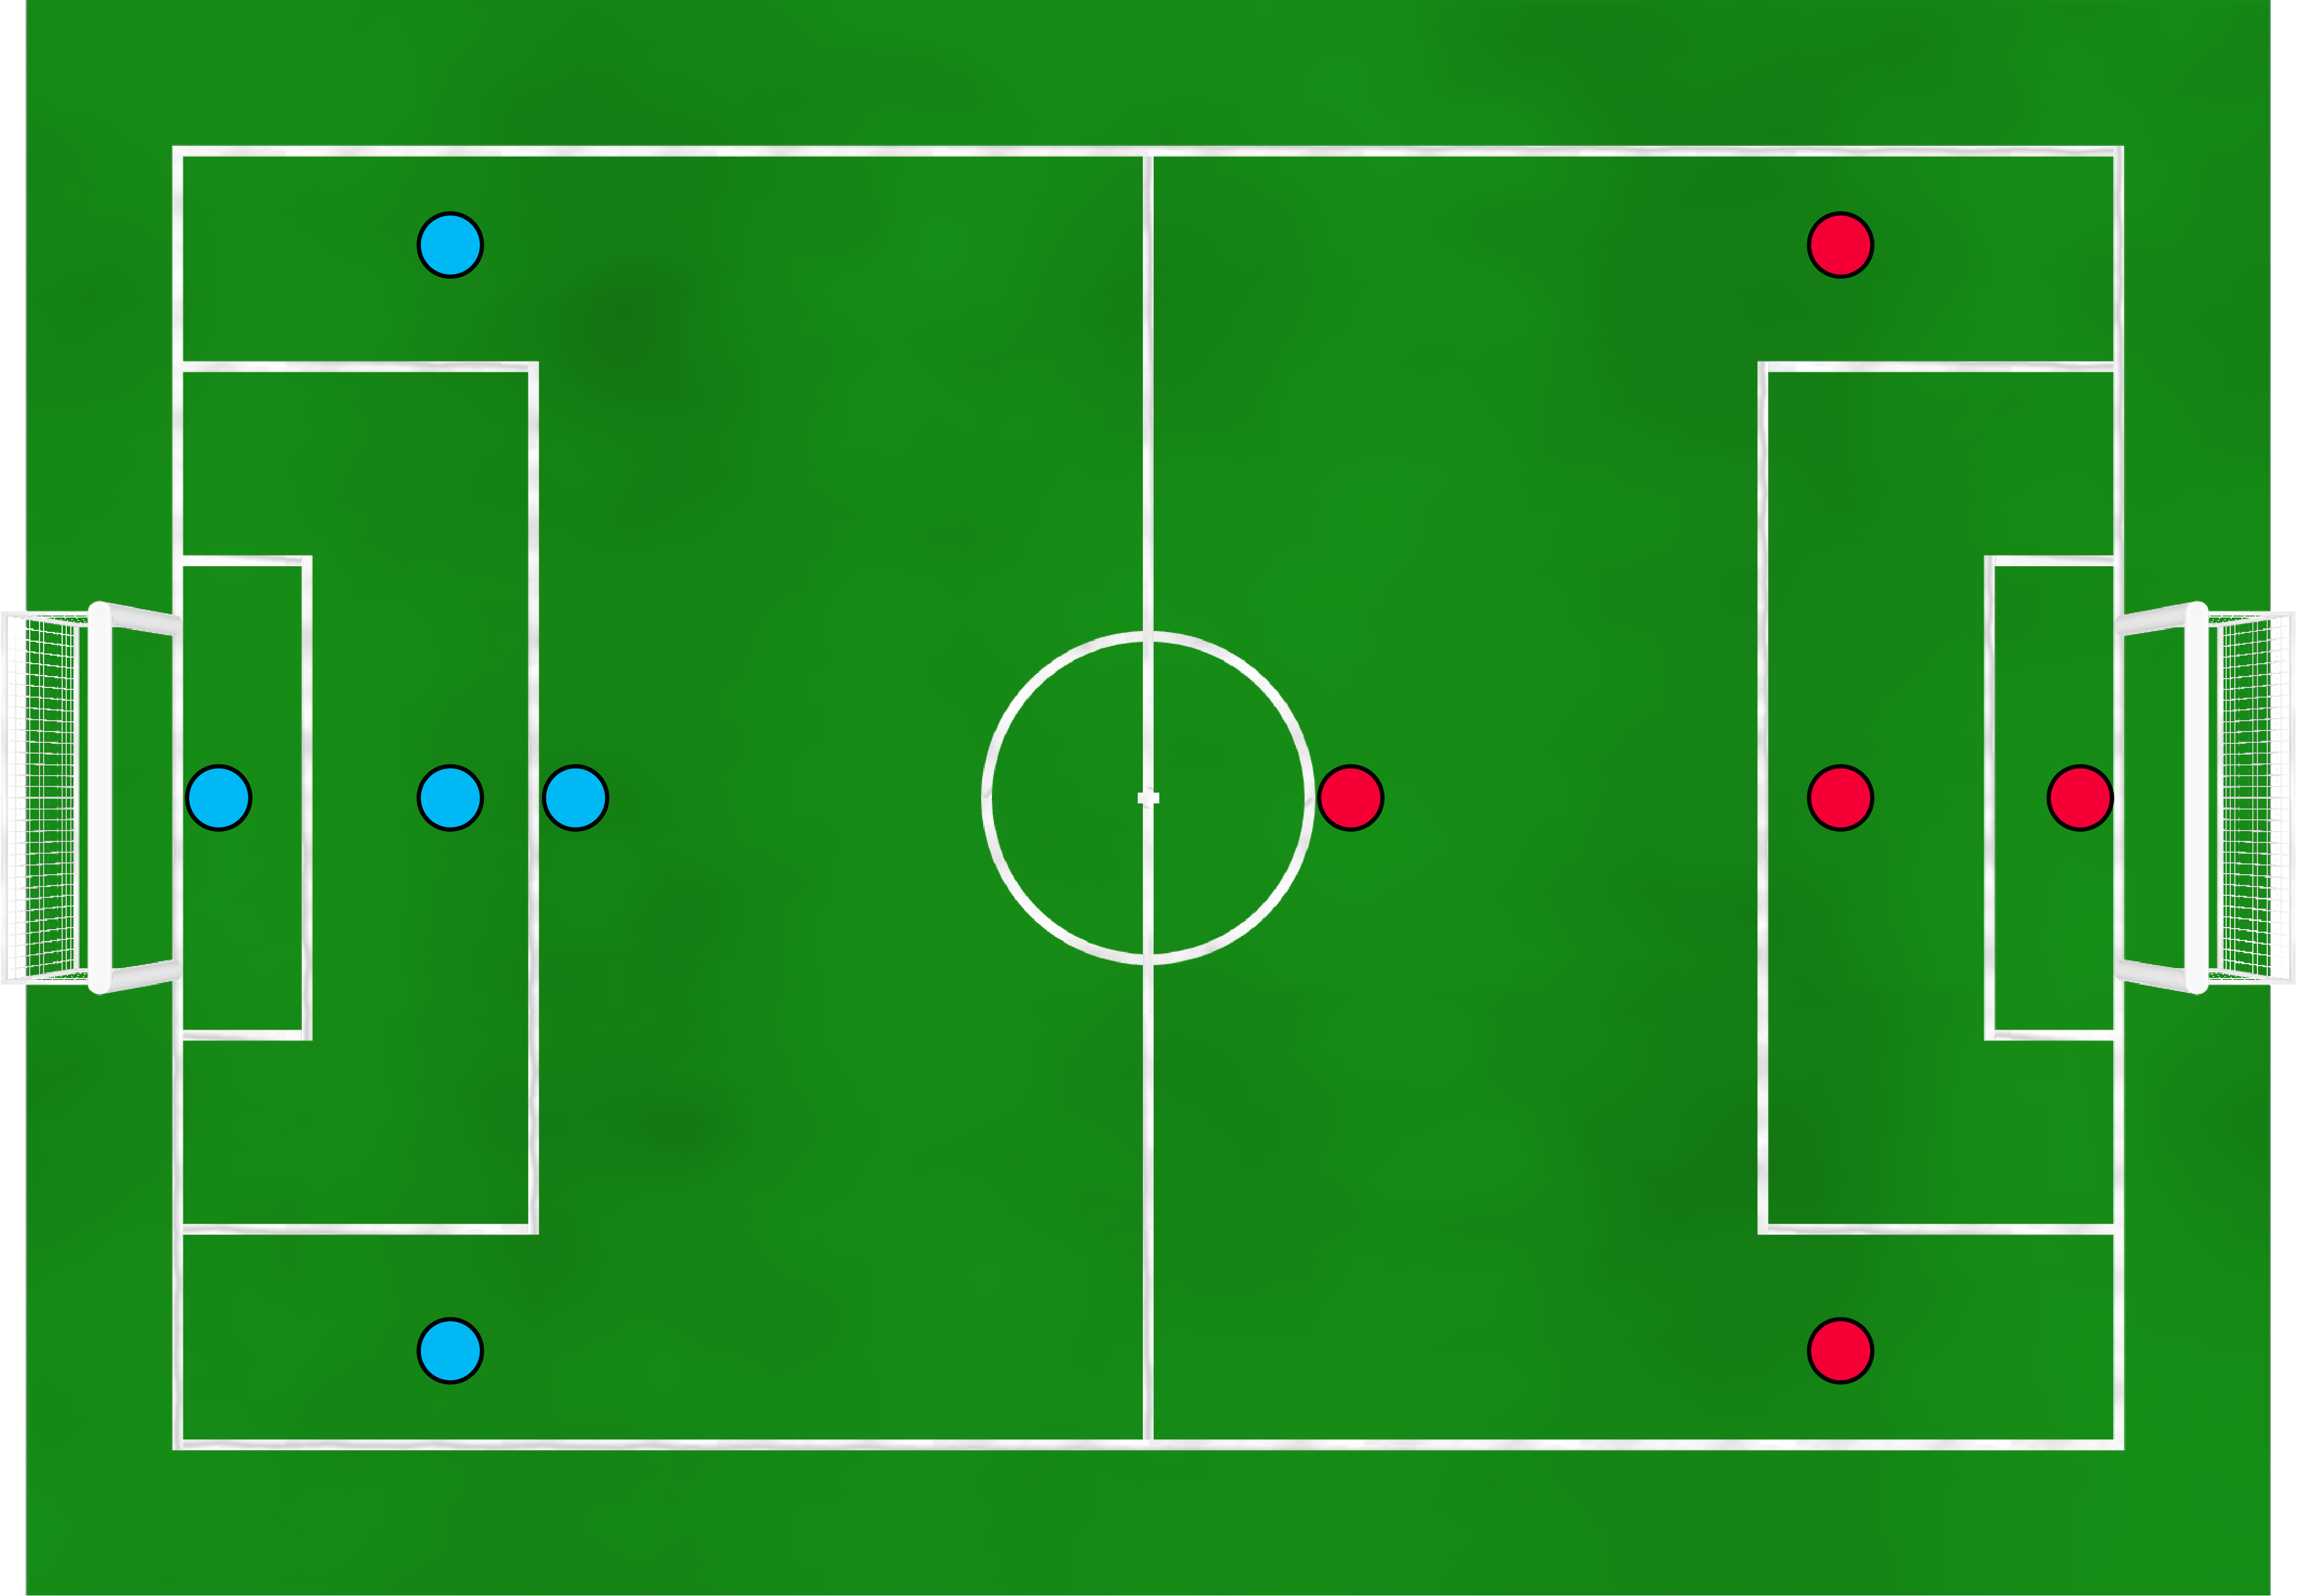
\includegraphics[width=\columnwidth]{figs/manual-placement-2020.png}}
%	\caption{Manual setup for kick-off.  The attacking team is on the right.}
%	\label{fig:ko}
%\end{figure}

%The positions for manually positioned robots are shown in Figure~\ref{fig:ko}. The kicking-off robot is placed such that its feet touch the center circle (but are not inside it), right in front of the penalty mark. The goal keepers for each team are placed at the center of the goal, with their feet immediately in front of the end-line.
%The other robots are positioned relative to the penalty spot, with one robot on the spot, and others outside of the penalty box.

%To assist the referees in placing the robots manually when needed or requested, small Xs will be marked on the field using a black felt-tip pen in the spots where manually placed robots should go.  These marks should be small, such that they are visible to humans but invisible to robots.

The head referee signals the kick-off by a single whistle blow, followed by the call ``Playing''. The head referee must signal this from the T-junction of the half-way line.

After the head referee has signalled the kick-off, the robot's state is switched to \emph{playing} by the GameController.

\paragraph{Kick-in}
\label{sec:kick_in}

A ball is considered to have left the field when there is no part of the ball over the outside of the boundary line (\ie the line itself is in). \\
If the ball goes over a sideline then the assistant referee will replace the ball back on the point of that sideline where it went out. \\
If the ball goes over an end-line then the assistant referee will replace the ball onto the corner of the goal box on the same side of the field that the ball was kicked-out. That is, the corner inside the field, not the t-junction where the goal box meets the goal line.
Note that no GameController action is required.

\paragraph{Global Game Stuck}
\label{sec:game_stuck:global}

In the event of no ``substantial change''\footnote{``substantial change'' can consist of a robot seeing and moving towards the ball OR robots exploring the field (presumably in an attempt to find the ball)} in the game state for 30 seconds OR or no ball was played from one half to the other for 1 minute, this is considered a global game stuck and the referee calls ``Global Game Stuck''. \\
Once the referee calls Global Game Stuck, players enter the Ready state, and a new kick-off (\cf Section~\ref{sec:kick-off}) is awarded.
\textcolor{red}{TODO:} Single GameController button for Global Game Stuck?


\paragraph{Request for Pick-up}
\label{sec:request_for_pickup}

Either team may request that their players be picked up (called ``Request for Pick-up'').
In the Playing or Ready state, players may only be picked up for hardware failures.
In all other states, players may be picked up for any reason.

Only hardware changes are allowed during a request for pick-up! In particular,
it is permitted to change batteries, fix mechanical problems, reboot the robots.
It is also allowed to replace a broken robot by a substitute robot.
However it is prohibited to change the robot's control program.

Any strategic ``Request for Pick-up'' is not allowed.
That is, gaining an advantage by removing the robot from the competition.
In this case, the head referee will indicate when the robot is no longer affecting play and can be removed from the field by an assistant referee.

To prevent mistakes and confusion during games, only team leaders should make a ``Request for Pick-up''.

The returning robot may be returned following the normal replacement procedure once at least 45 seconds have elapsed since the robot was removed from play. Note that this penalty does not follow the standard removal procedure, and hence does not count towards the incremental penalty count.

If the picked-up robot was penalized, the penalty time of the robot counts down with the game clock throughout the pick-up.
Note here, that the returning robot or the substitute robot will have to wait out any remaining penalty time of the picked up robot after the team handed their robot back to the assistant referees.
%TODO: RFP because of no Gamecontroller, automatic request for Pickup Referee,

\textcolor{red}{TODO}: Are the Assistants allowed to fix hardware problems (\ie reboot)?

\paragraph{Referee Timeout}
\label{sec:referee_timeout}
The head official may call a timeout at any stoppage of play if he or she deems it necessary. A referee timeout should only be called in dire circumstances --- one example might be when the power to the wireless router is down or no robot listens to the GameController. However, when and whether to call a referee timeout is left up to the head referee.

Referees may call multiple timeouts during a game if needed. Teams are only allowed to do hardware changes during these timeouts.  The referee should end the timeout once he or she believes the circumstance for which the timeout was called has been resolved.  In cases where the circumstance for which the timeout was called is not resolved within 10 minutes, the chair of the technical committee should be consulted regarding when/if play should continue.

\newpage

\subsubsection{Forbidden Actions and Penalties}
\label{sec:forbidden_act}

The following actions are forbidden. In general, when a penalty applies, the robot shall be replaced, not the ball.

\paragraph{Penalty Procedure}
\label{sec:penalty_procedure}

When a robot commits an infraction, the head referee shall call out the infraction committed, the primary jersey colour of the robot, and the jersey number of the robot. The penalty for the infraction will be applied immediately by an assistant referee. The assistant referees should perform the actual movement of the robots for the penalty so that the head referee can continue focusing on the game. The operator of the GameController will send the appropriate signal to the robots indicating the infraction committed.

For penalties that are timed, the penalty time is considered to be over at the end of each half.

\paragraph{Standard Removal Penalty}
\label{sec:removal_penalty}

Unless otherwise stated, all infractions result in the removal of the infringing robot from the field of play for a particular amount of time, after which it will be returned to the field of play. This process is called the \textit{standard removal penalty}.

When the head referee indicates an infraction has been committed that results in the standard removal penalty, the assistant referee closest to the robot will remove the robot immediately from the field of play. The robot should be removed in such a way as to minimize the movement other robots and the ball. If the ball is inadvertently moved when removing the robot, the ball should be replaced to the position it was in when the robot was removed.

The GameController will send the appropriate penalty signal to the robot indicating the infraction committed. After a penalty is signalled to the robot, it is not allowed to move in any fashion. The removed robot will be placed outside of the field facing away from the field of play.

The initial duration of the standard removal penalty time is \StandardPenaltyTime.
Unless otherwise specified, the penalty time increases by \StandardPenaltyIncrease each time a team commits any infraction.
That is, the first infraction will result in a penalty time of \StandardPenaltyTime, the second infraction (of any type) results in a penalty time of 55 seconds, the third infraction is 65 seconds, etc.

During the \emph{set} state the penalty time counter will not decrease.

The GameController will keep track of the time of the penalty. The operator of the GameController will signal the assistant referees when the penalty is 10 seconds from being over, so that one of them can place the robot in the half of the field which this robot's team is defending and on the sideline that is nearest to the GameController. The robot should be placed close to the position where the penalty spot projects on the sideline. This is illustrated in Figure~\ref{fig:penalty_re-entry_points}.

With approximately 5 seconds left before the penalty ends, the robot should be turned to face towards the opposite sideline.

\begin{figure}[t]
	\centerline{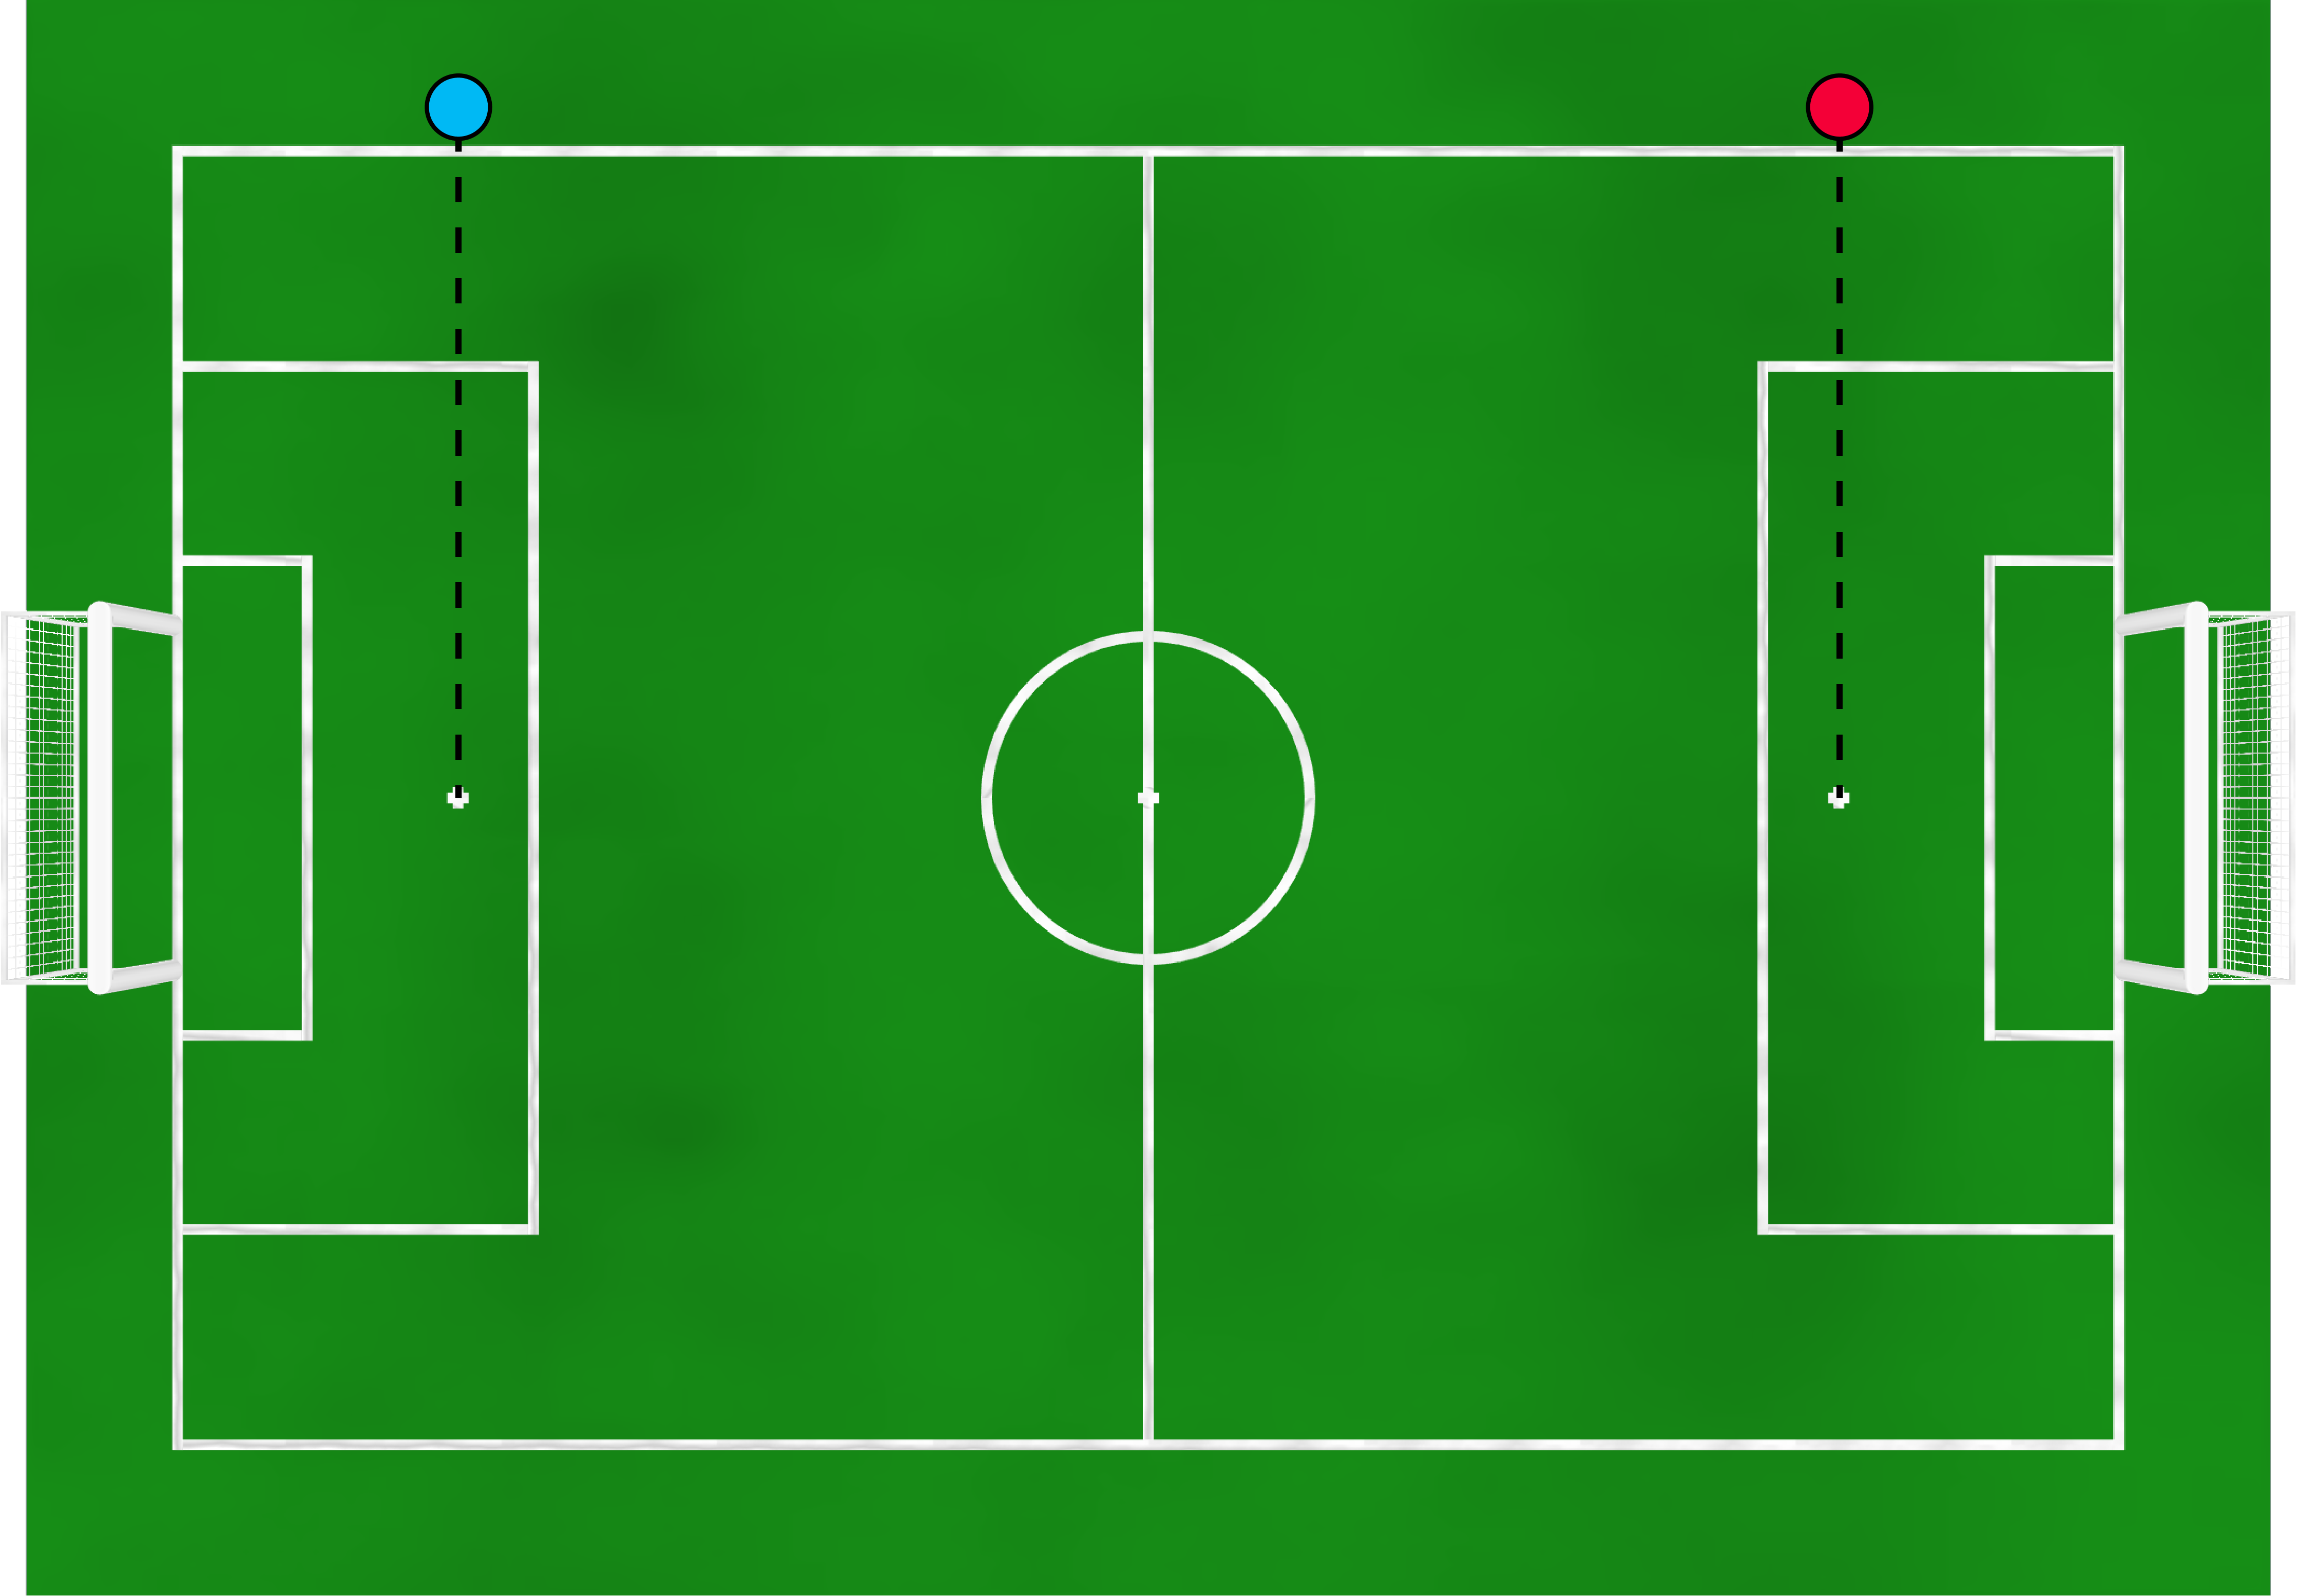
\includegraphics[width=\columnwidth]{figs/penalty_re-entry_points_2020.png}}
	\caption{For robots coming back from a standard removal penalty, re-entry points  are inline with the penalty spot in their own half, on the sideline on the side away from the ball.}
	\label{fig:penalty_re-entry_points}
\end{figure}

When the robot is on the field again, the operator of the GameController will send the \emph{playing} signal to it.

\paragraph{Forbidden Actions}

The following actions are forbidden, but not treated as penalties.
Each forbidden action specifies the actions to be taken by the referees.

\subparagraph{Manual Interaction by Team Members}

Manual interaction with the robots, either directly or via some communications mechanism, is not permitted.

\subparagraph{Locomotion Type}
\label{sec:locomotion_type}

Robots should clearly demonstrate bipedal walking similar to human walking. Other types of locomotion involving other parts than feet (crawling etc.) are strictly forbidden.
The head referee decides whether a robot's locomotion is appropriate. Robots using inappropriate locomotion types will be removed via ``Request for Pick-up'' until they are able to show appropriate locomotion.

\subparagraph{Damage to the Field}
\label{sec:damage}

A robot that damages the field, or poses a threat to spectator safety, will be removed from the field for the remainder of the competition.

\subparagraph{Damage to the Robot}
\label{sec:damage}

The head referee decides whether a robot excessively damages itself and should remove it from the field via ``Request for Pick-up''. 
All referees are allowed to prevent robots from crashing to the ground by catching them beforehand and then laying them down gently.
%TODO: Team scheidet aus, wenn Laufen so schlecht, dass es zwei Spiele lange nur hingefallen ist

\subparagraph{Illegal Positioning}
\label{sec:illegal_positioning}

A robot penalized under illegal position has the ``Illegal Position'' penalty applied. Illegally positioned robots are subject to the standard removal penalty (\cf Section~\ref{sec:removal_penalty}).
The head referee will call ``Illegal Position  \textless robot\textgreater''.

For simplicity, Illegal Positioning penalties during the \textit{Set} state (for kick-off) do not count towards the incremental penalty count\footnote{Historically, the Illegal Positioning penalty only occurred during a kick-off, and other illegal actions were termed Illegal Defender. Illegal Positioning \& Defender have been merged, but the penalty count left unchanged.}.

Refer to Section~\ref{sec:inside_outside} for the definition of \textit{inside/outside} of a region of the field.

``Illegal Position'' shall be imposed if a robot is not inside its own half at the time the Set state starts. It will then be penalized and removed for 15 seconds. The centre line does not count as part of the own half for this penalty, nor does the area inside the goal!

\paragraph{Motion in Set}
\label{sec:motion_in_set}

Robots may not exit the Set state until either the referee's whistle is detected or a GameController Playing signal has been received.
The head referee will call ``Motion in Set \textless robot\textgreater''.
The offending robot is penalized \textit{in-place} on the field. It will then be unable to move until it receives the GameController Playing signal. Motion in Set penalties do not follow the standard removal procedure, and hence do not count towards the incremental penalty count.

\paragraph{Fallen or Inactive Robots}
\label{sec:fallenrobots}

If a robot falls during the game, it should start executing a getup action within 5 seconds. If it does not commence a get up action within 5 seconds, it will be penalized and removed for \StandardPenaltyTime.
A robot which is unable to autonomously stand up within 20 seconds after a fall and be at least 10 seconds upright will be penalized and removed for \StandardPenaltyTime. 
In both cases, the head referee will call ``Fallen Robot  \textless robot\textgreater''.

\textbf{No robot} is permitted to `dive' (that is deliberately fall in a way that might cause its torso, arms or hands) to intercept the ball. The robots should be programmed to attempt to remain upright -- that is, supported by its feet.

A robot that has ceased activity for 10 seconds or has turned off will be removed and penalized for 45 seconds.
The head referee will call ``Inactive Robot  \textless robot\textgreater''.
A robot is active if it performs at least one of the following:
\begin{enumerate}
	\item The robot walks in any direction, or turns.
	\item The robot searches for the ball, or is looking at the ball.
\end{enumerate}

Fallen/Inactive Robot penalties do not follow the standard removal procedure, and hence do not count towards the incremental penalty count.

\subparagraph{Note:} The intention of this rule is not to penalize robots simply for being stationary -- provided they are not `asleep' and have not `crashed'.

\paragraph{Player Stance}
\label{sec:player_stance}

\textcolor{red}{TODO:} Allow wide stance to intercept a ball?

%Robots are not allowed to stay in a stance that is wider than the width of the robot's shoulders for more than 5 seconds. The robot is allowed to go into a wide stance as long as it comes back to a normal stance within 5 seconds. Staying in a wide stance for longer than 5 seconds will result in the standard removal penalty. If the robot has fallen down, it must start getting up within 5 seconds.

\paragraph{Playing with Arms/Hands}
\label{sec:hand_ball}

Playing with arms/hands occurs when a field player moves its arms/hands to touch the ball (except during a fall or get-up). A robot playing with arms/hands will be subject to the standard removal penalty and the ball will be replaced at the point where it contacted the arms/hands of the offending robot. If an own goal is scored as a result, the goal should count and the player should not be penalized.

Accidental playing with arms/hands when a robot falls or executes a get-up routine will not be penalized. 
If the ball goes out of play in this case, normal kick-in rules will apply (\cf Section~\ref{sec:kick_in}). 
Goals resulting from a ball contact with the arms/hands during a fall or get-up do not count and result in a kick-in (\cf Section~\ref{sec:kick_in}) as if the ball went over the goal line next to the goal.

\paragraph{Leaving the Field}
\label{sec:leaving_field}

A robot that intends to leave the \TotalWidth $\times$ 3.7~m\xspace carpeted area of its \textbf{own half} will be subject to the standard removal penalty (\cf Section~\ref{sec:removal_penalty})! A touching/exceeding of the centre/halfway line also leads to this standard removal penalty. 
The head referee will call ``Leaving the Field \textless robot\textgreater''.

Additionally, a robot will also be subject to the standard removal penalty when:
\begin{itemize}
	\item the robot walks into the goal posts or into the goal area for more than 5 seconds, this includes robots that are stuck on the goal posts and unable to free themselves
	\item the robot's finger become entangled in the net (without any time constraint).
\end{itemize}

\subsubsection{Judgment}

The referees are the only persons permitted on the carpeted area (\ie the field and the border area).

The local team of an arena has to provide the referees. The number of referees depends on local regulations and can be reduced to a head referee and an operator of the GameController.

All referees are allowed to prevent robots from crashing to the ground by catching them beforehand and then laying them down gently!

\paragraph{Head Referee}
\label{sec:head_referee}

The head referee is in charge of the game. Any decision of the head referee is valid. The head referee's decision is final and can not be changed afterwards, even by video proof. There is no discussion about decisions during the game, neither between the assistant referees and the head referee, nor between the audience/spectators or the teams and the head referee.

The head referee also decides whether a robot excessively damages itself and should be removed from the field (\cf Section~\ref{sec:damage})

The head referee announces decisions by a clear loud call, and (as required) whistle sound.
The whistle, or where there is no whistle the first verbal word of the referees calls, defines the point in time at which the decision is made.
The referees should make efforts to use consistent and clear calls, and it is preferable for referees to use the calls as specified in these rules\footnote{The calls specified in these rules are detailed in English. With the agreement of the teams, the referees may use suitable calls in any language. The exception to this are technical challenge(s) that depends on the calls as specified.}.
The intention of specifying the referee calls is for clarity and consistency across games.

Where a whistle is required, the head referee first whistles and then announces the reason for the whistle.
The head referee may choose to use any normal sports whistle.
Each whistle sound should be short and not too loud.
The head referee must \textit{only} sound the whistle in circumstances described in these rules.
There are three circumstances when the whistle is sounded, Kick-off~(\cf Section~\ref{sec:kick-off}), a goal~(\cf Section~\ref{sec:goal}), and ending a half of gameplay~(\cf Section~\ref{sec:game_struct}).

The head referee should avoid handling the ball (except for placing the balls for a kick-off), and avoid handling the robots.
Their duty is to monitor and adjudicate the game.
The head referee should only handle robots and the ball if absolutely necessary to expedite gameplay or removal of penalized robots, where the assistant referees are otherwise occupied, are too far away or had to be dropped.

\paragraph{Assistant Referees}
\label{sec:assist_referee}
The, in the ideal case, two assistant referees handle the robots and the ball. They start the robots if the wireless is not working, they move the robots, if manual placement is requested, they take the robots out when they are penalized, and they put the robots in again. An assistant referee will also put the robot back on the field. An assistant referee will also replace the ball when it goes off the field or becomes stuck between a players feet.

If a team requests to pick up a robot, an assistant referee will pick it up and puts it on the sideline. Also the assistant, on behalf of the teams, can do hardware changes to robots on the sideline, \ie reboot it or change and secure the battery. 

The assistant referees can \textit{indicate} violations against the rules committed by robots to the head referee, so that the head referee can decide whether to penalize a certain robot or not. Assistant referees should only enter the field to execute a decision made by the main referee or to catch a falling robot.

\paragraph{Operator of the GameController}
\label{sec:gameControllerOp}
The operator of the GameController sits at a PC outside the playing area.
As with the head referee, the operator should make efforts to use consistent and clear calls.
They will signal any change in the game state to the robots via the wireless as they are announced by the head referee.
Note that for both kick-offs and goals, the moment of whistling is determining, not the verbal announcement of the head referee.
The operator will also inform the assistant referees when a timed penalty is over and a robot has to be placed back on the field.
They should announce when the ball is in play on kick-off by stating ``Ball Free'', if the \KickOffBallFreeTime time period has elapsed in the playing state.
They are also responsible for keeping the time of each half (\ie, they stop the clock after a global game stuck, and continues it at the kick-off).
They should count aloud the remaining seconds in a half once the time remaining is 5 seconds or less.
Finally, they should repeat the calls of the head referee to make sure it was heard correctly.

\paragraph{Referees During the Match}

The head referee and the assistant referees should wear clothing and socks \emph{of black or dark blue colour} (blue jeans are acceptable) and avoid reserved colours for the ball, the goals, and player markings in their clothing. They may enter the field in particular situations, \eg, to remove a robot when applying a penalty. They should avoid interfering with the robots as much as possible.

\subsection{A Remark on Artificial Landmarks}
\label{sec:judgment:landmarks}

The head referee may decide at any point before or during a game to relocate any objects around the field, or direct persons to another position around the field.

The intent of using same-coloured goals is to remove artificial landmarks.
Robots should be able to localize with the SPL field and its ``normal'' surroundings.
Introducing new team-specific artificial landmarks is against the spirit and intention of the league's progress.
The application of this rule needs to be well considered and should be reserved for situations which seem constructed by one team or another, but will ultimately be the head referee's decision alone.

\newpage

% Arne
6. Points will be counted by the referees and not by the GC.
7. Points can be scored by:
    - Shooting the ball in opponents half and it stops there (1 Point)
    - Shooting a goal (not own goal) (1 Point)
    - Touching the opponents player with the ball (0 Point)
11. Teams playing with an autonomous player get a scoring factor of 2. Each point is multiplied by this factor.

\subsection{Challenge execution}
% Arne
The clock stops during stoppages of play (such as ready and set state after global game stuck)!

\subsubsection{Winner and Rankings}
\label{sec:rankings}

The team which scored more points, after the expiration of the regular playing time, than the other is the winner of the match. If the two teams scored the same number of points, the game will be a draw. In case of a draw the game duration gets extended by one minute. After each extension the score is evaluated again. At max 5 extensions are allowed. 
\textcolor{red}{TODO}: Final determination? Coin toss?


- Ladder system
- KO system 
- groups of 8 teams per Ladder
- randomly assignment of teams to groups
- losers of a match will play in additional ladders (To allow all teams to play at least 3 times)
- Winners play games against each other
- Time zones (Two games per day)
- can only be finalized when the exact number of participants is known
    
\newpage

\subsection{Field Technical Drawings}
\label{apx:technical-drawing}
\centerline{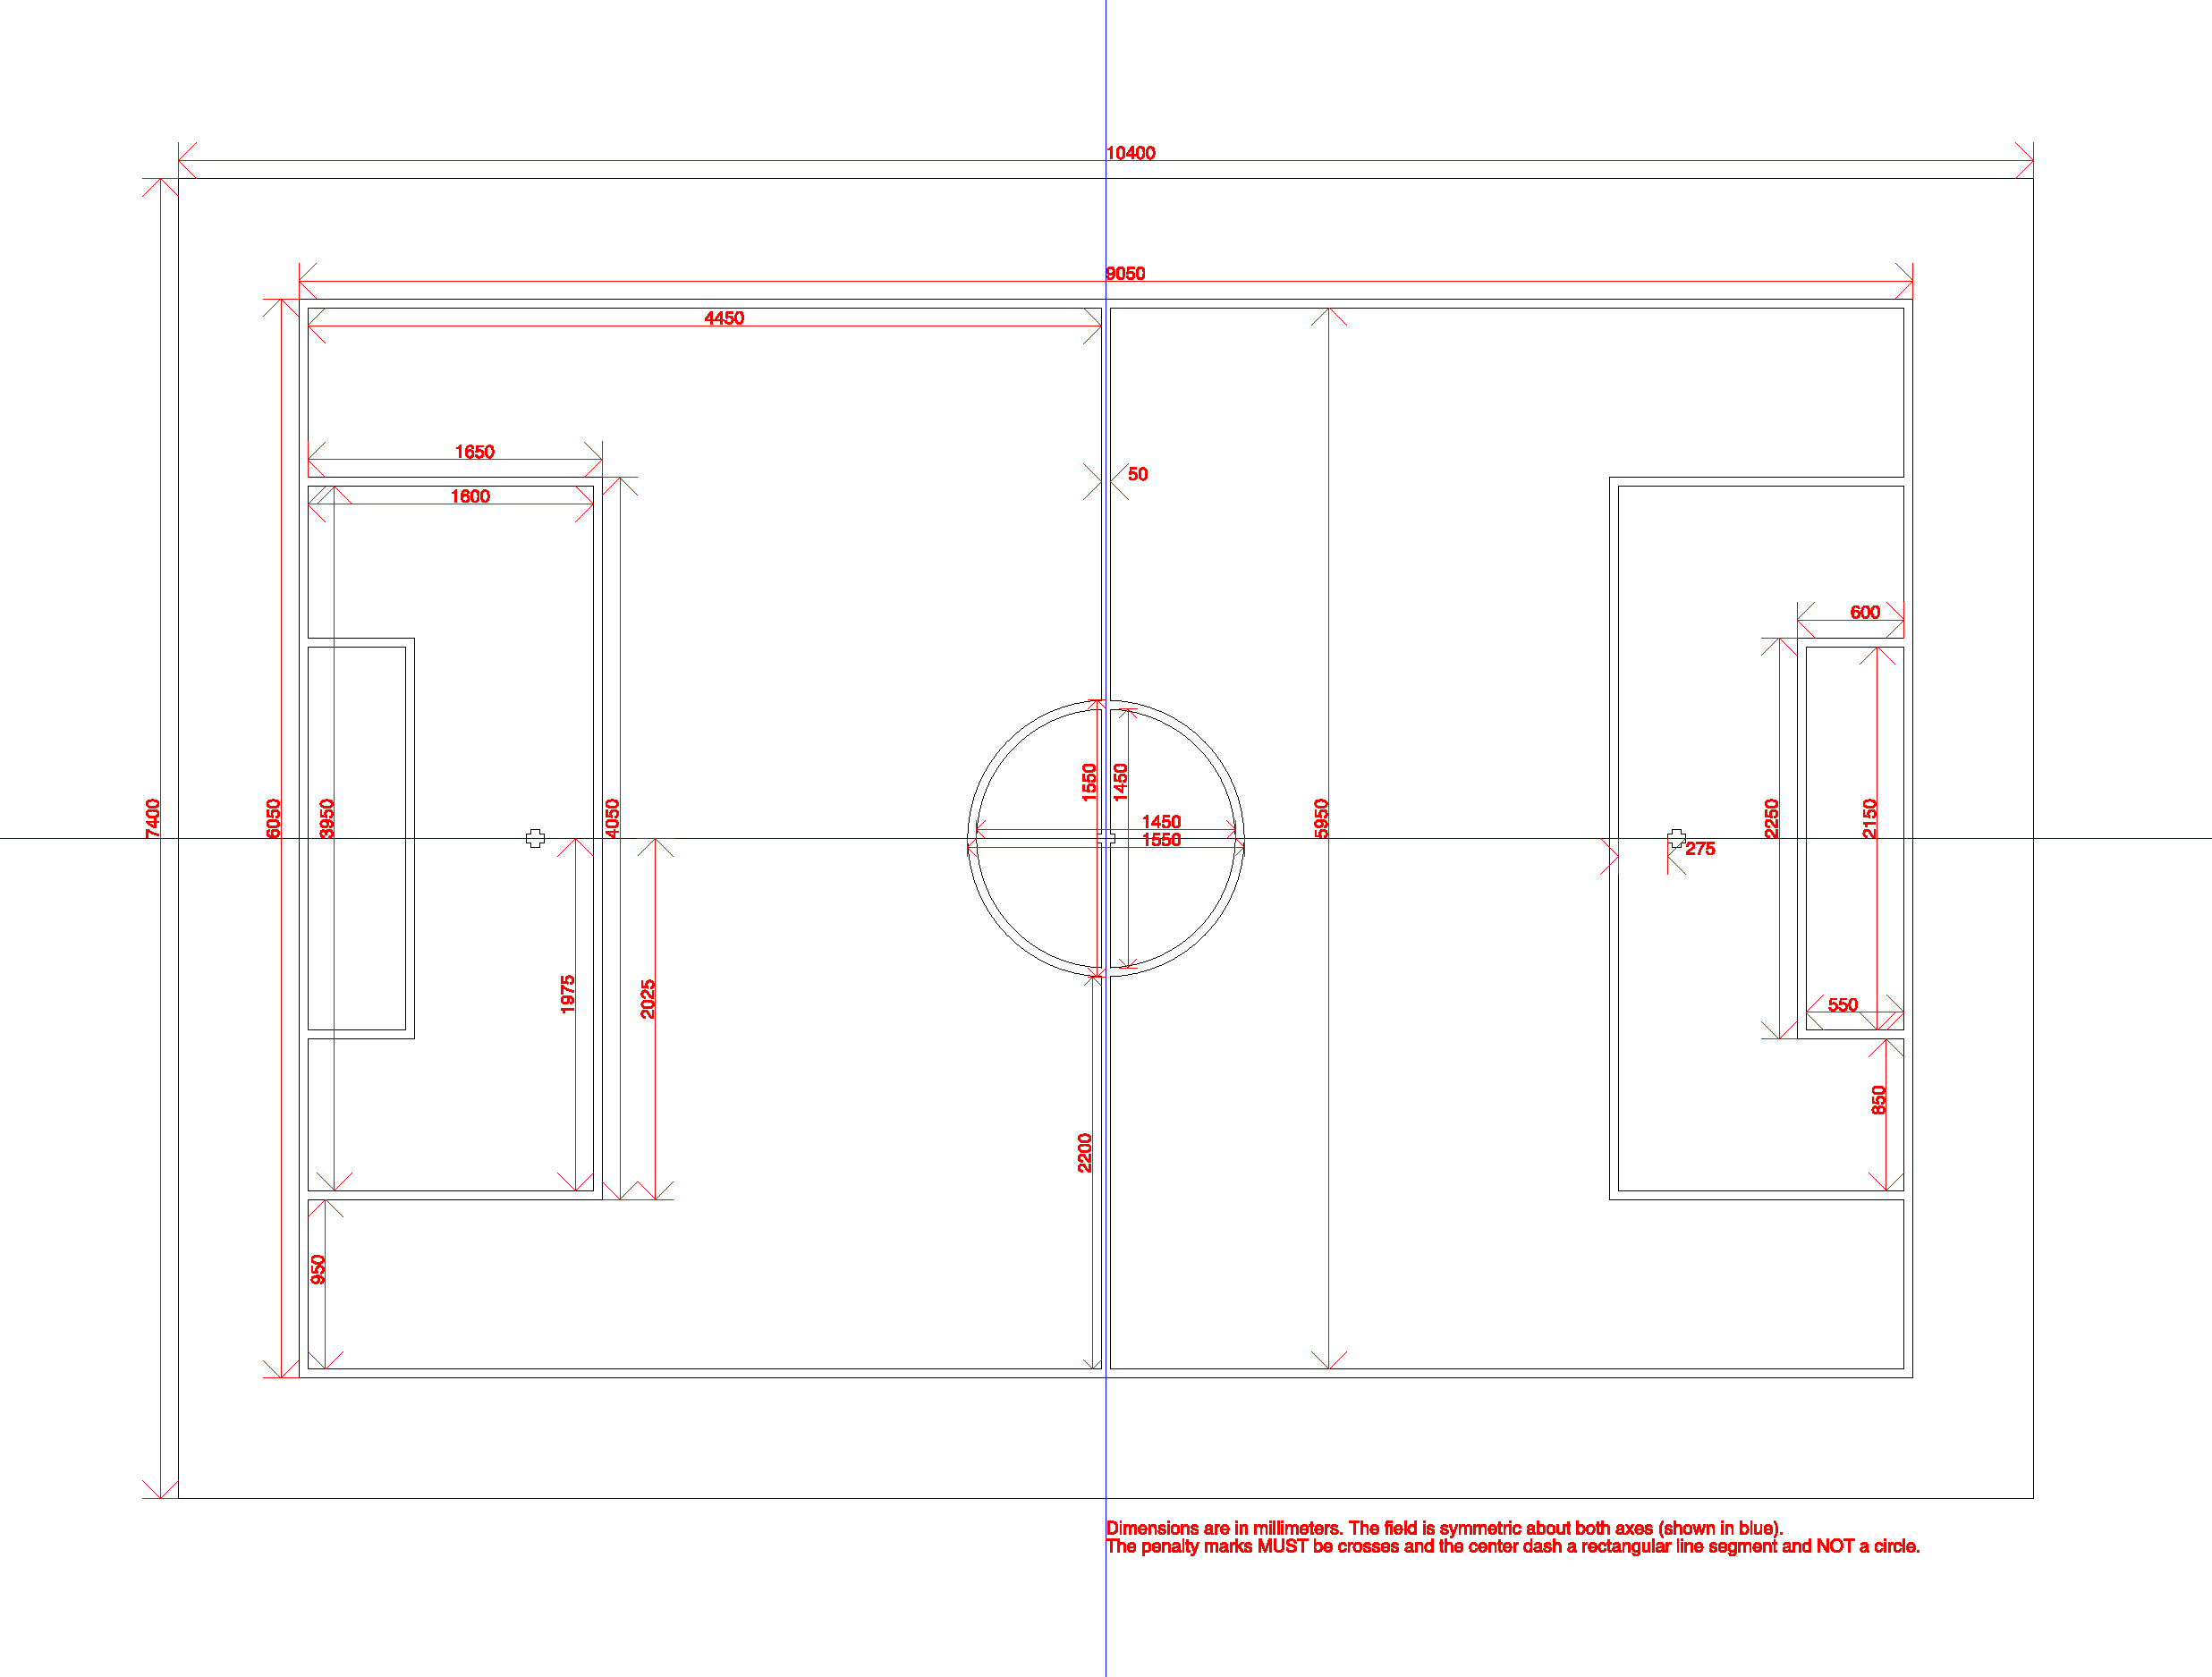
\includegraphics[angle=90,origin=c,width=\columnwidth]{figs/fieldDimensions2020_technical.pdf}}

\clearpage
%\textbf{Center Circle}
\centerline{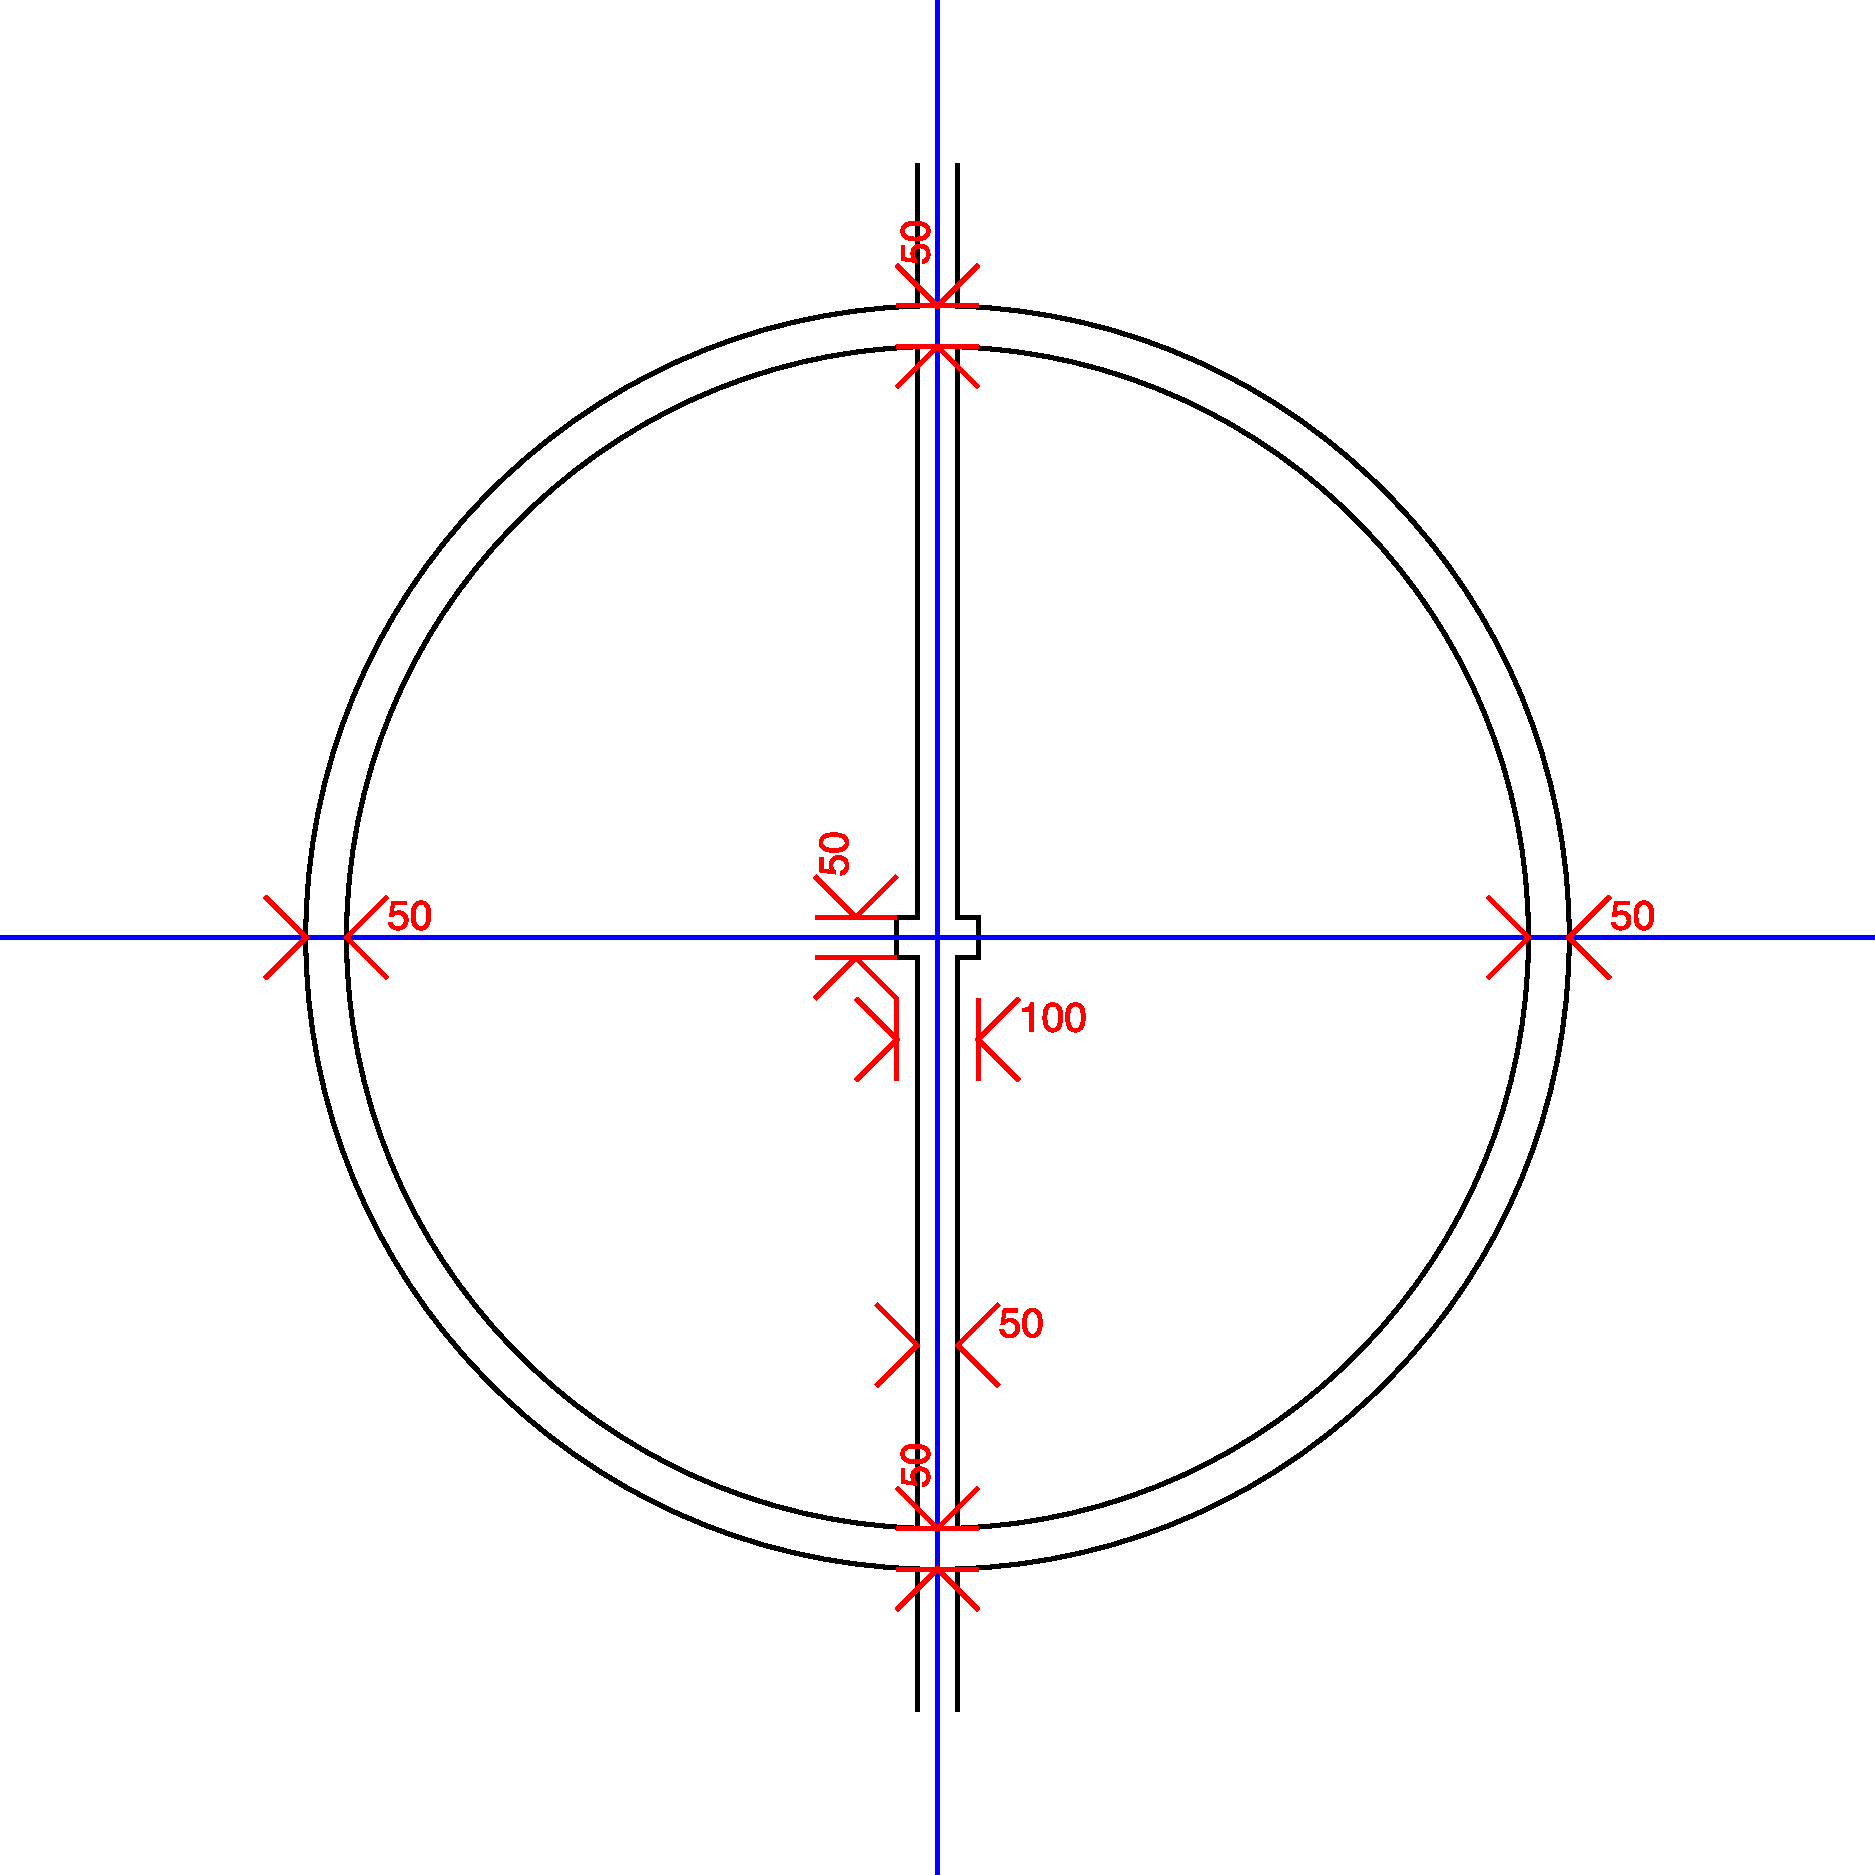
\includegraphics[angle=90,origin=c,width=0.5\columnwidth]{figs/fieldDimensions2020_technical_cc.pdf}}

\centerline{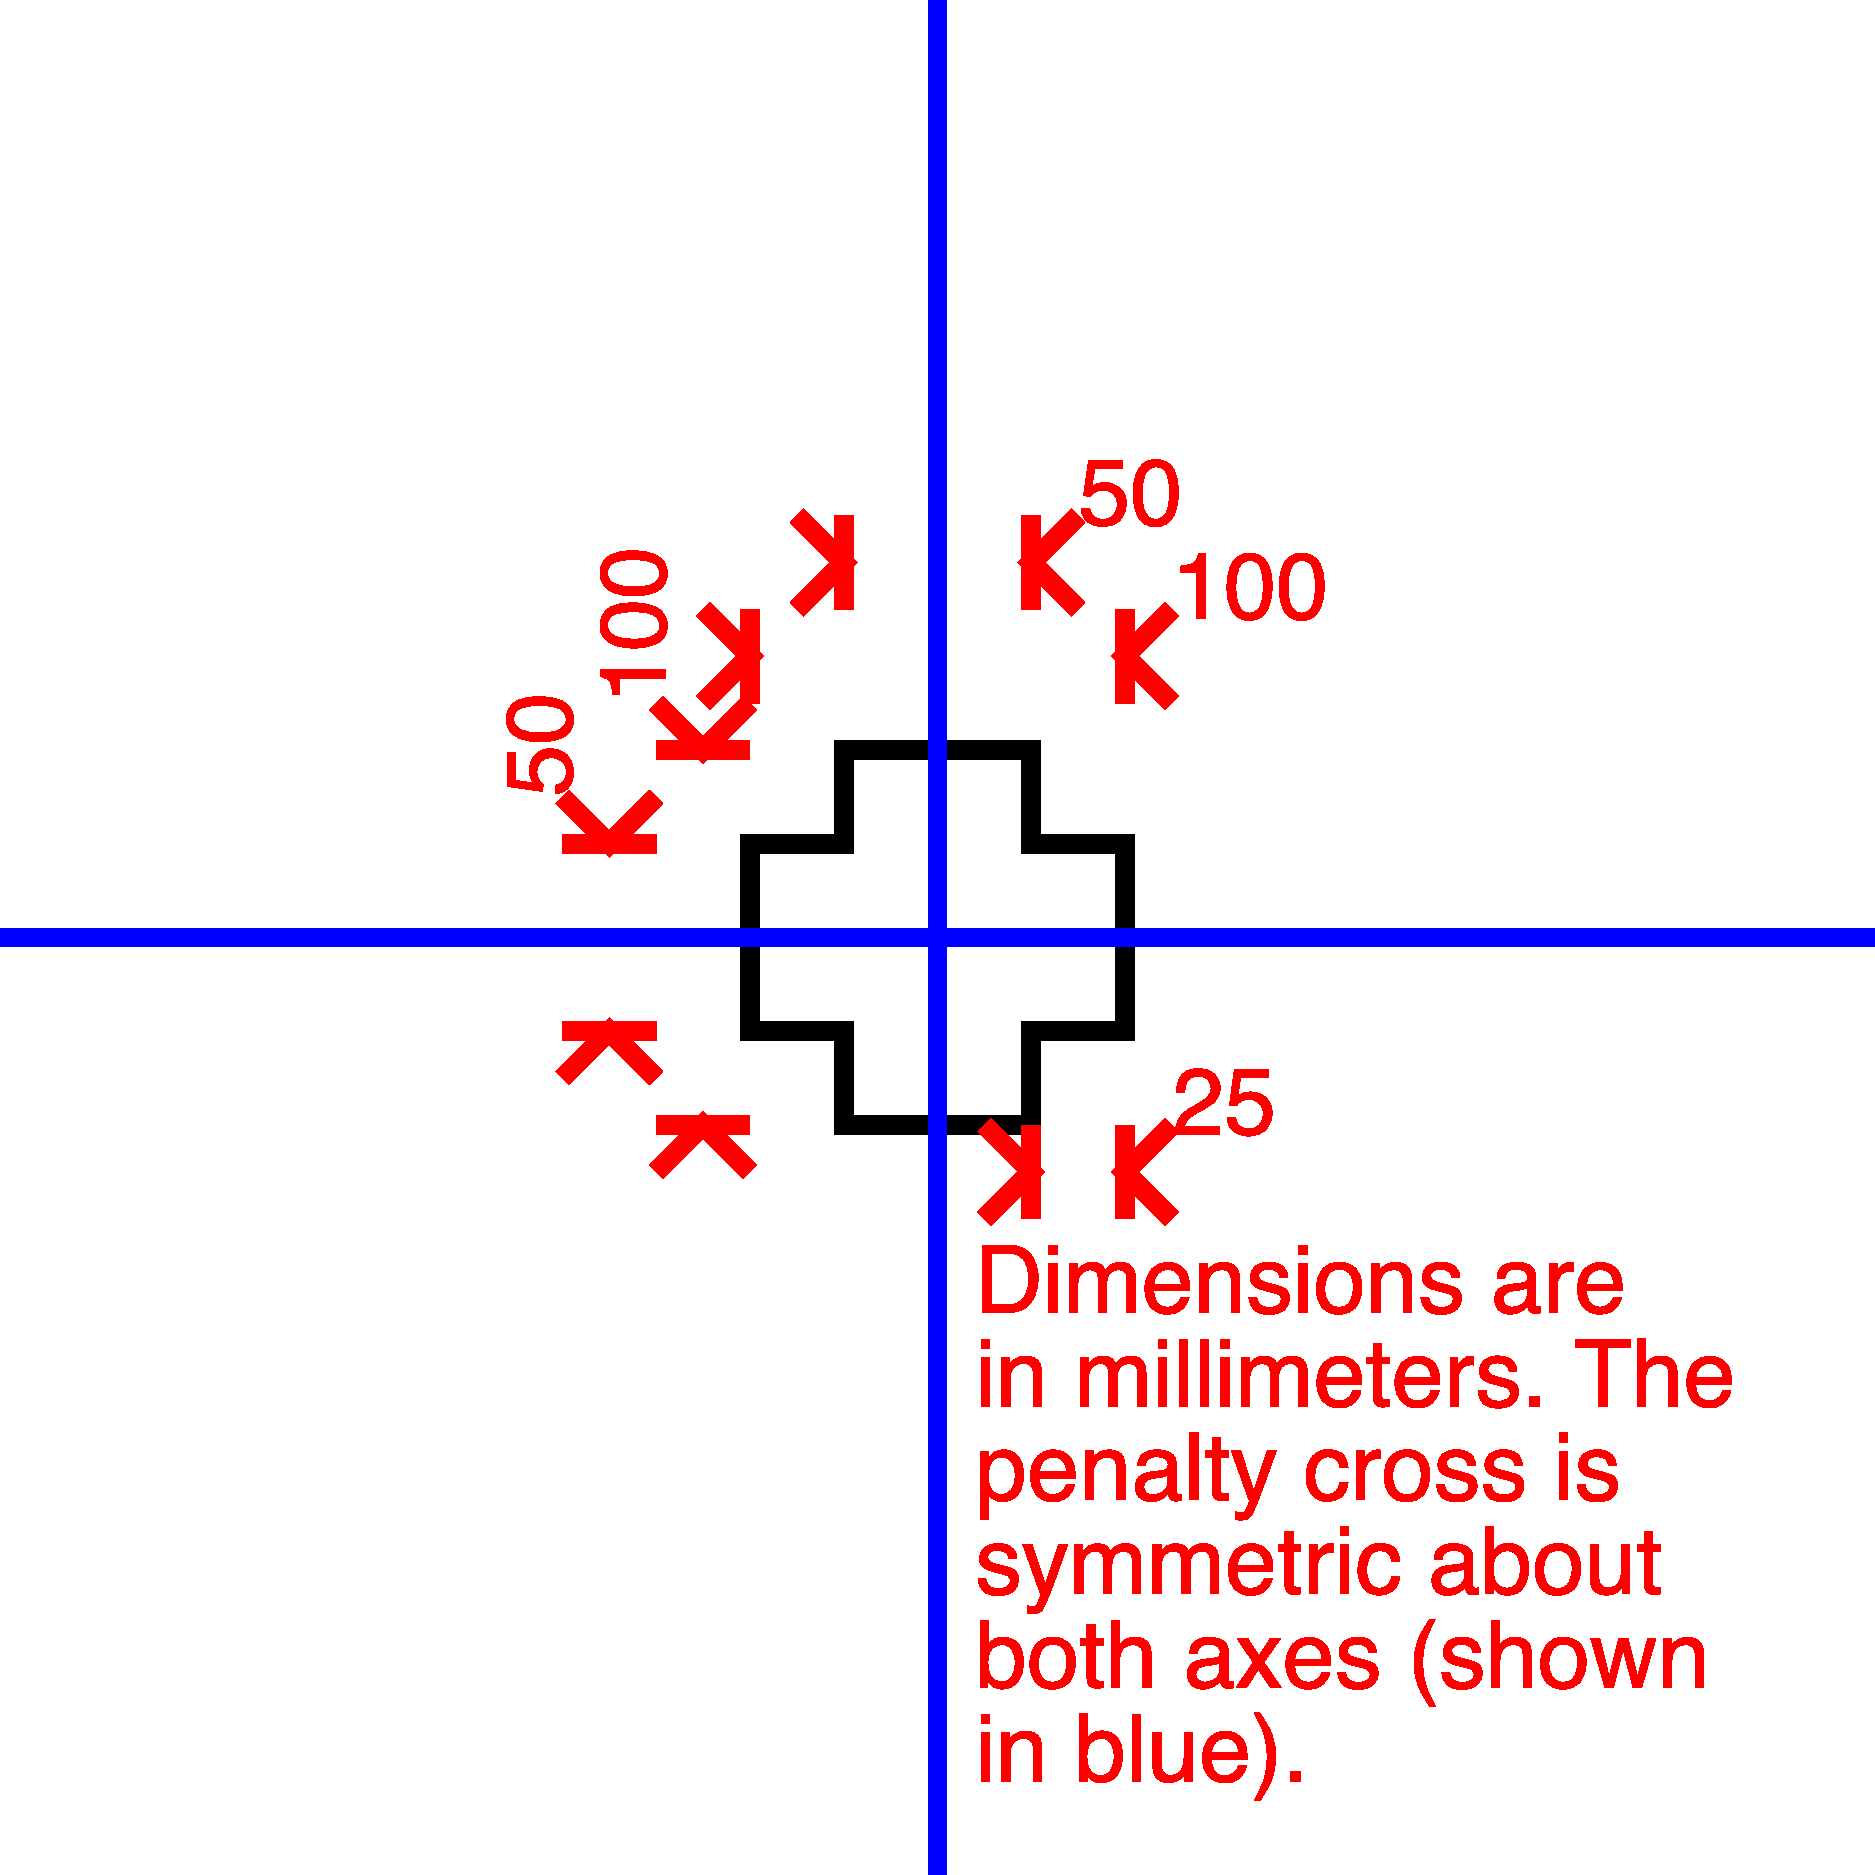
\includegraphics[origin=c,width=0.5\columnwidth]{figs/fieldDimensions2020_technical_pc.pdf}}

%\change{Add the figures for Center Circle and penalty cross as well.}